\documentclass[]{book}
\usepackage{lmodern}
\usepackage{amssymb,amsmath}
\usepackage{ifxetex,ifluatex}
\usepackage{fixltx2e} % provides \textsubscript
\ifnum 0\ifxetex 1\fi\ifluatex 1\fi=0 % if pdftex
  \usepackage[T1]{fontenc}
  \usepackage[utf8]{inputenc}
\else % if luatex or xelatex
  \ifxetex
    \usepackage{mathspec}
  \else
    \usepackage{fontspec}
  \fi
  \defaultfontfeatures{Ligatures=TeX,Scale=MatchLowercase}
\fi
% use upquote if available, for straight quotes in verbatim environments
\IfFileExists{upquote.sty}{\usepackage{upquote}}{}
% use microtype if available
\IfFileExists{microtype.sty}{%
\usepackage{microtype}
\UseMicrotypeSet[protrusion]{basicmath} % disable protrusion for tt fonts
}{}
\usepackage[margin=1in]{geometry}
\usepackage{hyperref}
\hypersetup{unicode=true,
            pdftitle={CannaData 0.0.0.900 Documentation},
            pdfauthor={Carl Ganz},
            pdfborder={0 0 0},
            breaklinks=true}
\urlstyle{same}  % don't use monospace font for urls
\usepackage{natbib}
\bibliographystyle{plainnat}
\usepackage{longtable,booktabs}
\usepackage{graphicx,grffile}
\makeatletter
\def\maxwidth{\ifdim\Gin@nat@width>\linewidth\linewidth\else\Gin@nat@width\fi}
\def\maxheight{\ifdim\Gin@nat@height>\textheight\textheight\else\Gin@nat@height\fi}
\makeatother
% Scale images if necessary, so that they will not overflow the page
% margins by default, and it is still possible to overwrite the defaults
% using explicit options in \includegraphics[width, height, ...]{}
\setkeys{Gin}{width=\maxwidth,height=\maxheight,keepaspectratio}
\IfFileExists{parskip.sty}{%
\usepackage{parskip}
}{% else
\setlength{\parindent}{0pt}
\setlength{\parskip}{6pt plus 2pt minus 1pt}
}
\setlength{\emergencystretch}{3em}  % prevent overfull lines
\providecommand{\tightlist}{%
  \setlength{\itemsep}{0pt}\setlength{\parskip}{0pt}}
\setcounter{secnumdepth}{5}
% Redefines (sub)paragraphs to behave more like sections
\ifx\paragraph\undefined\else
\let\oldparagraph\paragraph
\renewcommand{\paragraph}[1]{\oldparagraph{#1}\mbox{}}
\fi
\ifx\subparagraph\undefined\else
\let\oldsubparagraph\subparagraph
\renewcommand{\subparagraph}[1]{\oldsubparagraph{#1}\mbox{}}
\fi

%%% Use protect on footnotes to avoid problems with footnotes in titles
\let\rmarkdownfootnote\footnote%
\def\footnote{\protect\rmarkdownfootnote}

%%% Change title format to be more compact
\usepackage{titling}

% Create subtitle command for use in maketitle
\newcommand{\subtitle}[1]{
  \posttitle{
    \begin{center}\large#1\end{center}
    }
}

\setlength{\droptitle}{-2em}
  \title{CannaData 0.0.0.900 Documentation}
  \pretitle{\vspace{\droptitle}\centering\huge}
  \posttitle{\par}
  \author{Carl Ganz}
  \preauthor{\centering\large\emph}
  \postauthor{\par}
  \date{}
  \predate{}\postdate{}

\usepackage{booktabs}
\usepackage{amsthm}
\makeatletter
\def\thm@space@setup{%
  \thm@preskip=8pt plus 2pt minus 4pt
  \thm@postskip=\thm@preskip
}
\makeatother

\usepackage{amsthm}
\newtheorem{theorem}{Theorem}[chapter]
\newtheorem{lemma}{Lemma}[chapter]
\theoremstyle{definition}
\newtheorem{definition}{Definition}[chapter]
\newtheorem{corollary}{Corollary}[chapter]
\newtheorem{proposition}{Proposition}[chapter]
\theoremstyle{definition}
\newtheorem{example}{Example}[chapter]
\theoremstyle{definition}
\newtheorem{exercise}{Exercise}[chapter]
\theoremstyle{remark}
\newtheorem*{remark}{Remark}
\newtheorem*{solution}{Solution}
\begin{document}
\maketitle

{
\setcounter{tocdepth}{1}
\tableofcontents
}
\chapter{Preliminaries}\label{preliminaries}

The CannaData platform enables Marijuana dispensaries to manage their
patients, inventory, point-of-sales, and online presense with one
integrated platform. Each client receives a seperate Virtual Private
Cloud instance where their data is securely stored. When you create an
account with CannaData you will be given a unique url for your
dispensary. For example, a dispensary named ``storename'' would likely
receive the domain \url{https://storename.cannadata.com} where they can
securely access the CannaData platform.

An elegent, and up-to-date menu is readily available at
\url{https://storename.cannadata.com/menu}, which can easily be
integrated into your dispensaries webpage.

CannaData is not simply a piece of software. We are your go-to data, and
technology consultant. Once your dispensary is integrated into our data
pipeline, we over a variety of custom business services including
reporting/analytics, A/B testing for marketing campaigns, patient
surveys, and more.

This documentation explains how to use the CannaData platform's 4
primary applicaitions.

\section{Contact}\label{contact}

We love getting feedback! Please email
\href{mailto:carl@cannadatasolutions.com}{Carl Ganz}

\chapter{Frontdesk}\label{frontdesk}

The Frontdesk is where every dispensary first makes contact with their
patrons. Dispensaries must keep track of all patrons, and verify that
they are valid medical marijuana patients. This requires checking-in
each patron when they enter the store. The CannnaData Frontdesk
application provides facilities for:

\begin{itemize}
\item
  Checking-in patients
\item
  Adding new patients
\end{itemize}

\section{Returning Patients}\label{returning-patients}

For returning patients, the front desk is responsible for:

\begin{itemize}
\item
  Validating the returning patient is who they say they are
\item
  Making sure their medical card is still valid
\item
  Controlling how many patients are allowed in the store at one time,
  and making sure that patients are processed in the correct order
\end{itemize}

All patient interactions begin by scanning the patient's state issued
ID. For returning patients this will pull up the patient's profile where
the budtender can quickly see the patient's current medical status, as
well as other basic information about the patient.

\begin{figure}
\centering
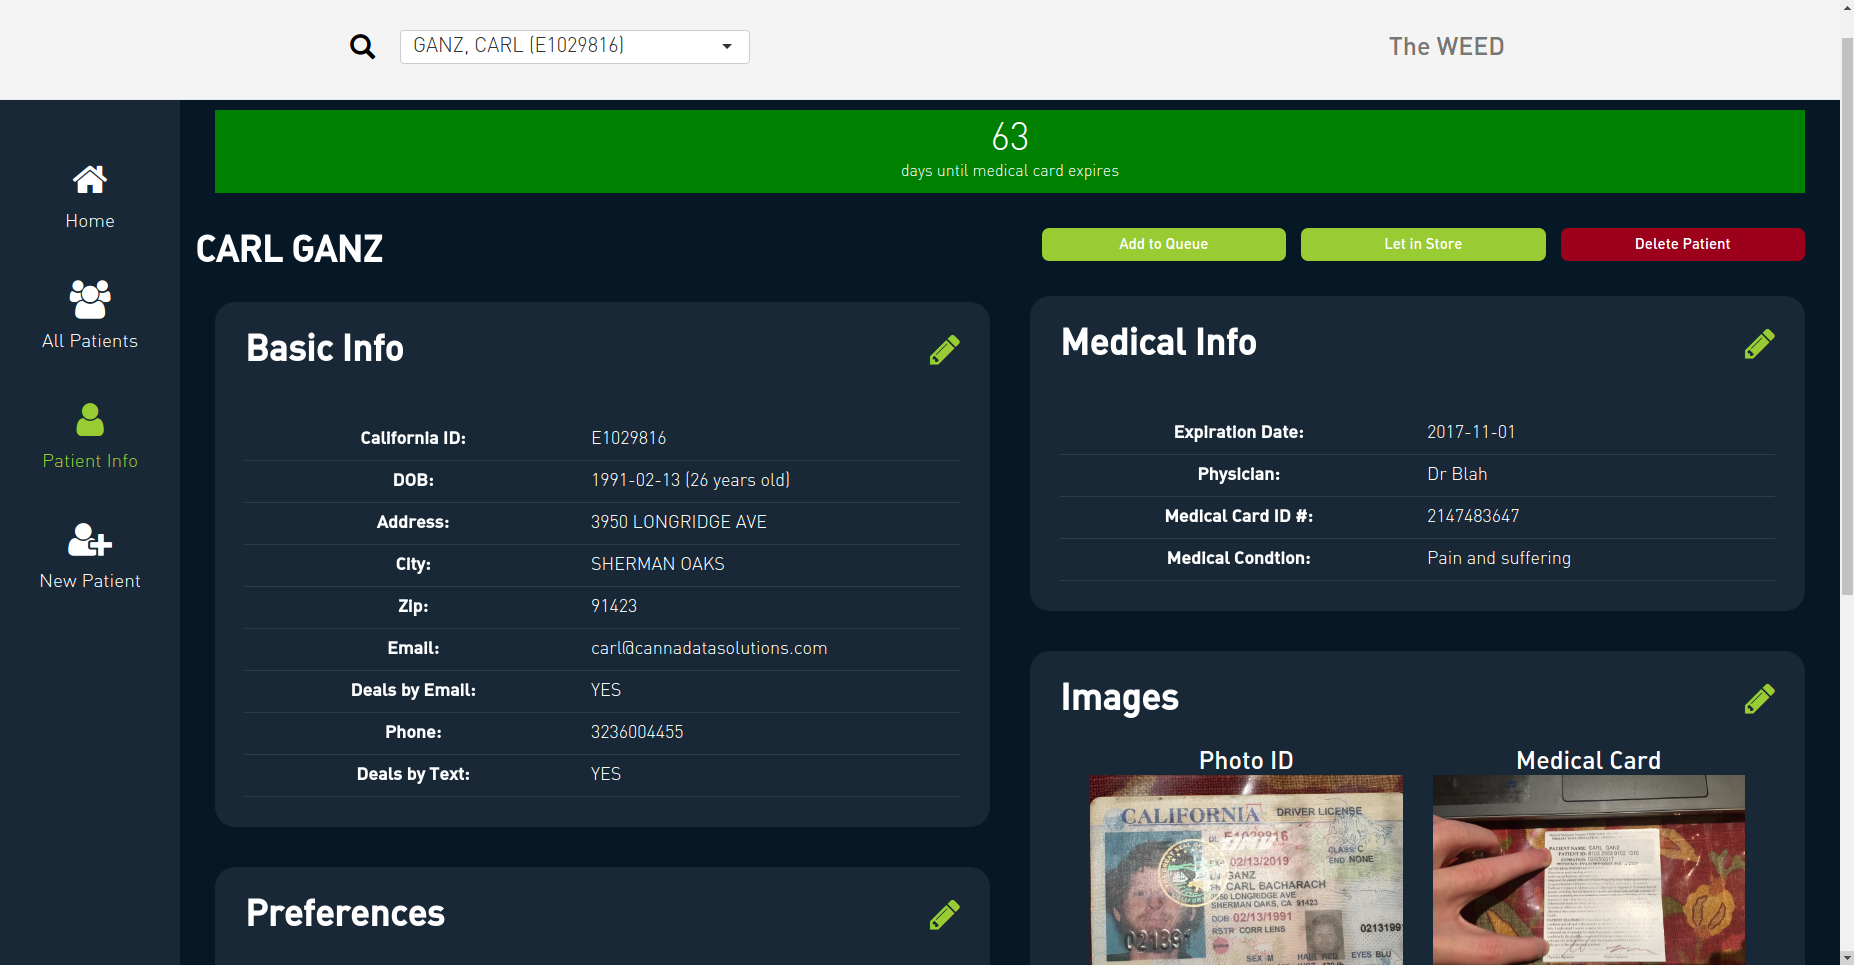
\includegraphics{images/FD1.png}
\caption{Returning Patient Info}
\end{figure}

\textbf{(NOTE TO NAYELI: I don't know if the images are placed optimally
in the patient info page. I tried this alternative set-up that may have
potential but didn't really work out as I hoped. I'd appreciate your
thoughts here.)}

\begin{figure}
\centering
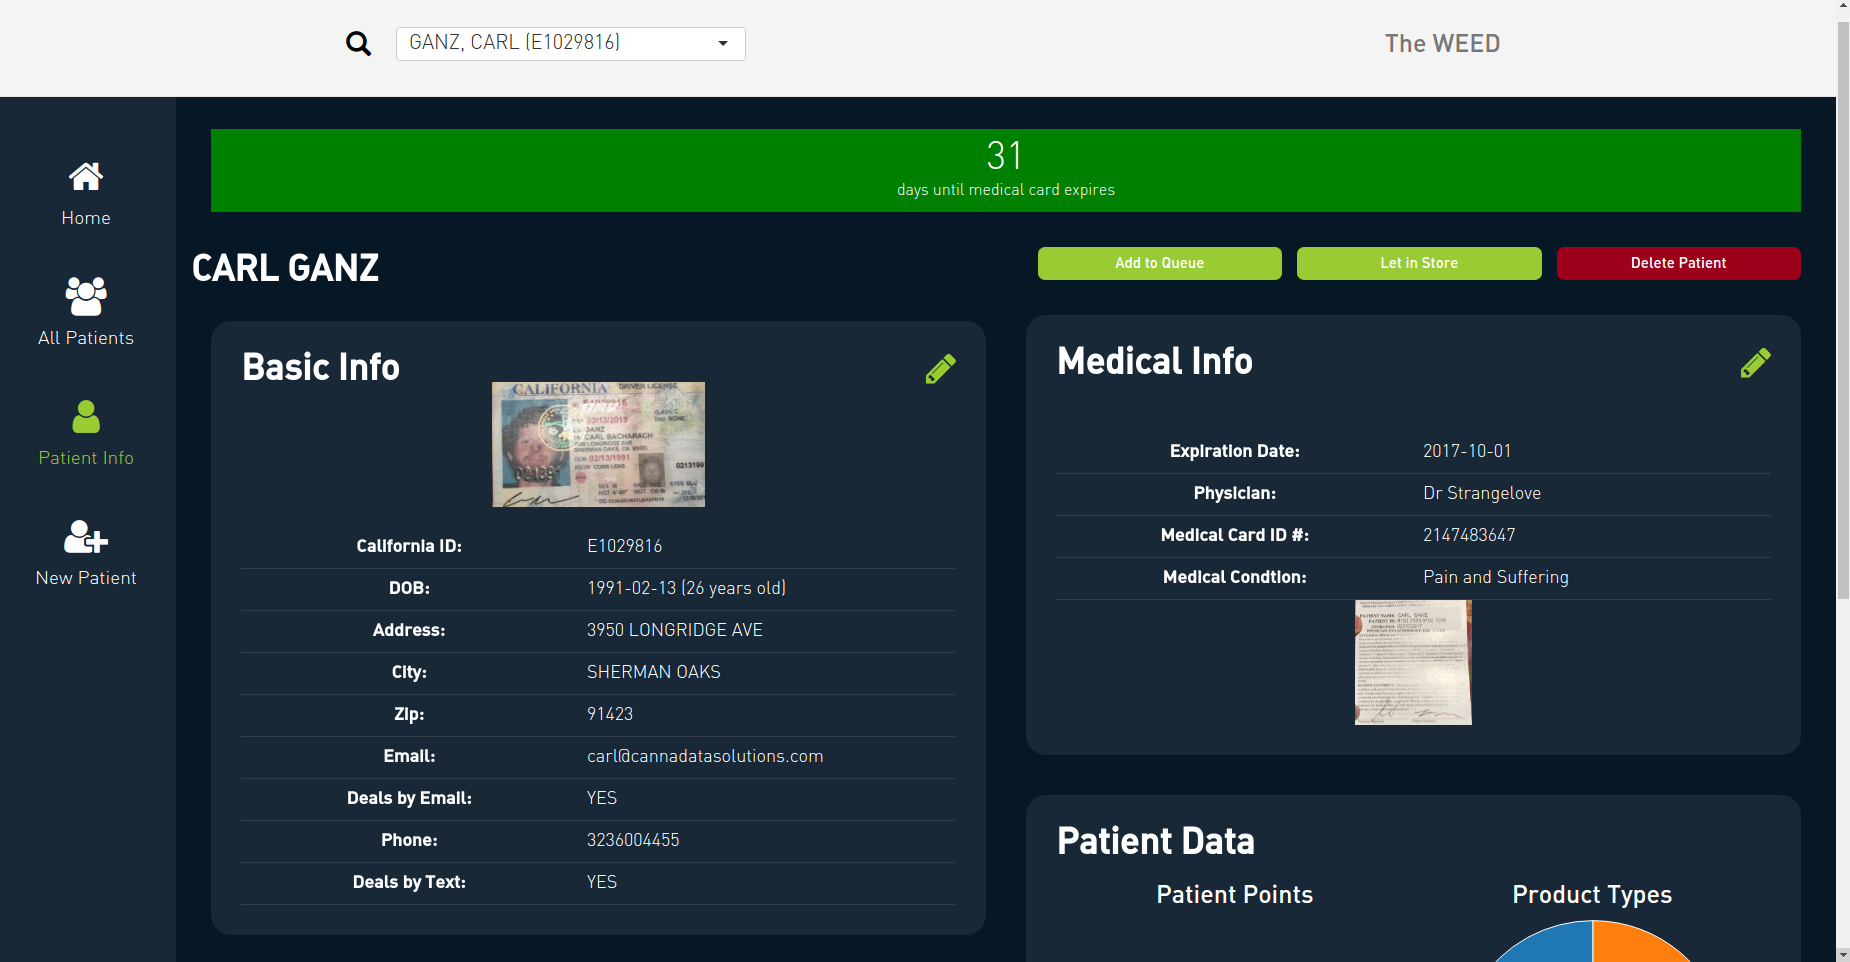
\includegraphics{images/FDalt.png}
\caption{Alternative Returning Patient Info}
\end{figure}

This makes it easy to verify that the patient's medical card is still
valid. You can also access a patient's info page by either searching for
them in search box in the top, or by selecting them from the All
Patients table.

\begin{figure}
\centering
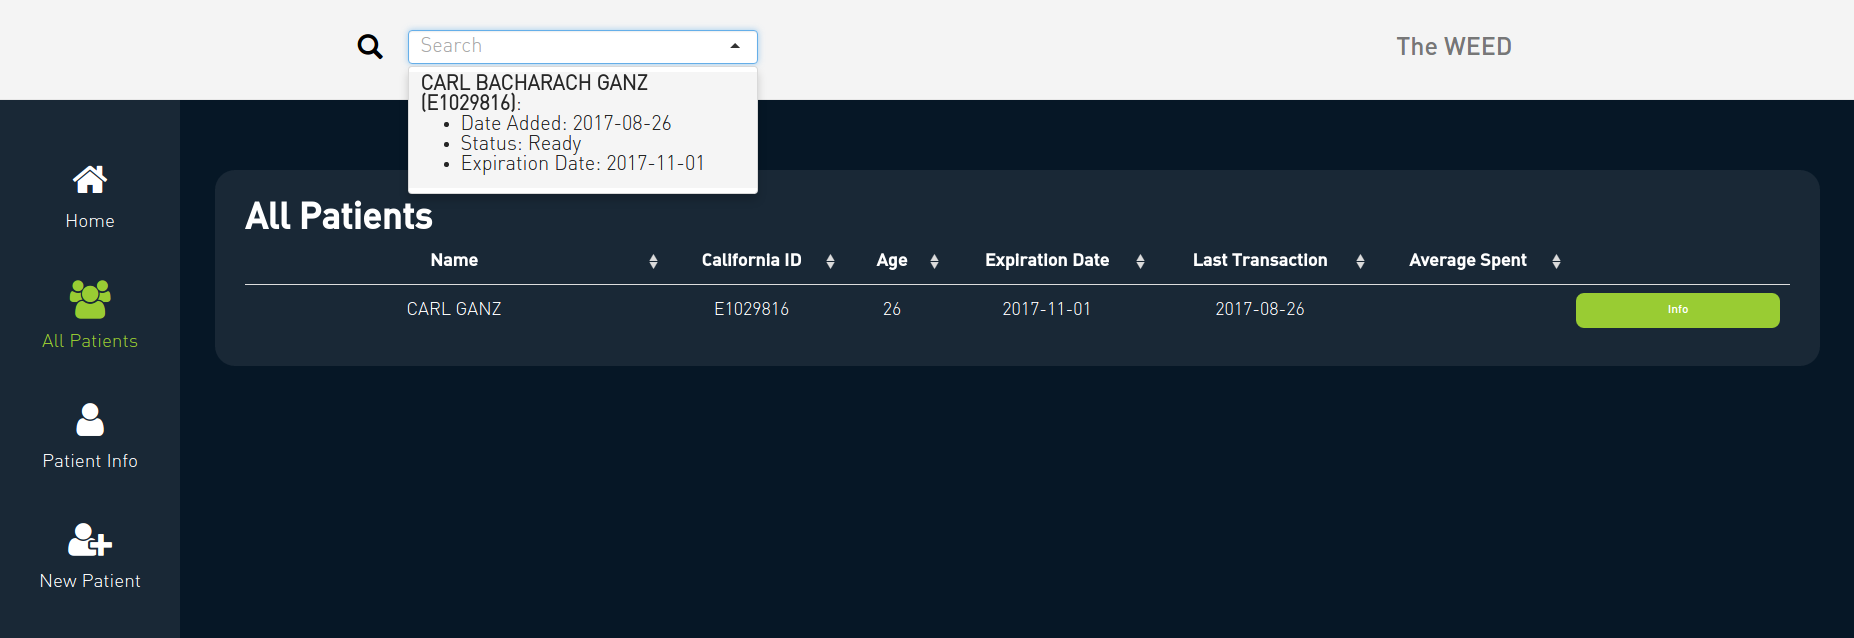
\includegraphics{images/FD3.png}
\caption{All Patient Table}
\end{figure}

For valid patients, the budtender has buttons at the top that allow them
to let the patient directly into the store, or if there is a line to get
in to the store, they can add the patient to a queue.

\begin{figure}
\centering
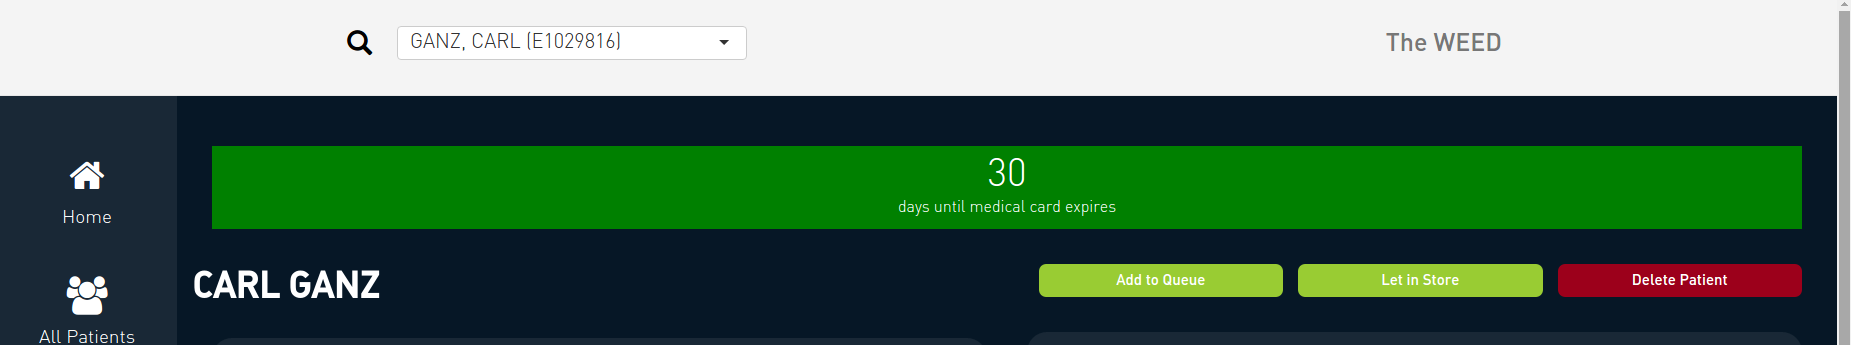
\includegraphics{images/FD12.png}
\caption{Returning Patient Buttons}
\end{figure}

\subsection{Queue}\label{queue}

The homepage of the Frontdesk app keeps track of who is currently in the
store, and who is currently in line to get in the store (queue). These
tables make it easy to see who is next in line, and how long people have
been waiting.

\begin{figure}
\centering
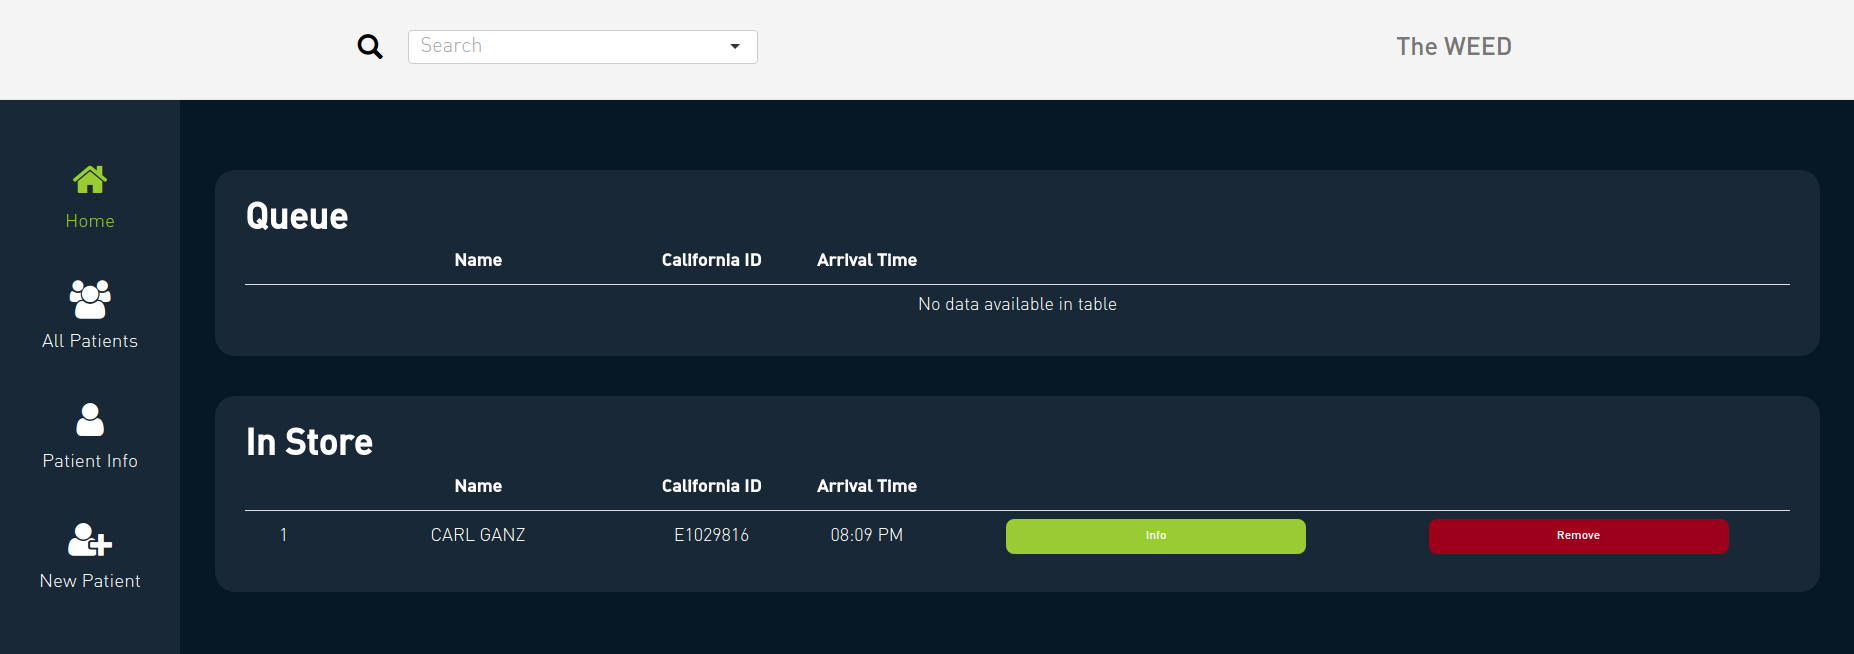
\includegraphics{images/FD2.png}
\caption{Queue}
\end{figure}

\subsection{Charts}\label{charts}

The patient info page provides charts and tables that are useful to the
budtender. This includes:

\begin{itemize}
\item
  The number of reward points the patient has accumulated (and how many
  more points they need to get a prize)
\item
  Which types of products the patient has bought in the past
\item
  Details of past transactions
\end{itemize}

\begin{figure}
\centering
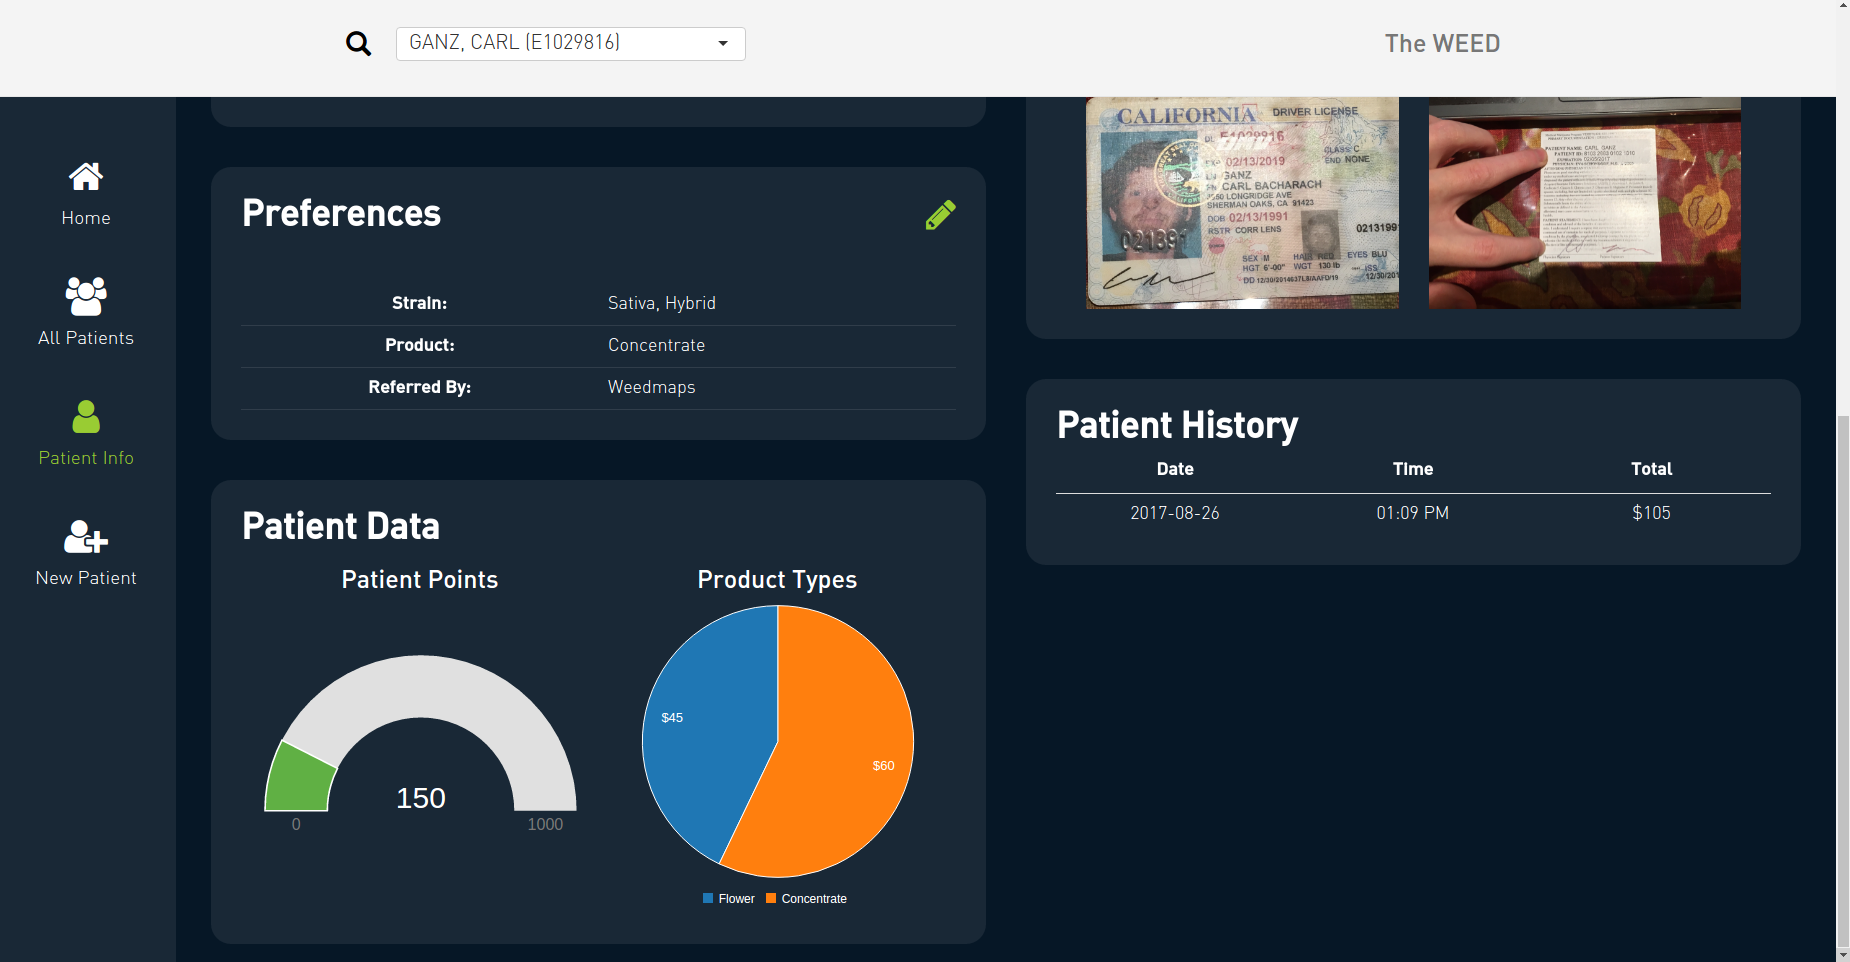
\includegraphics{images/FD4.png}
\caption{Charts}
\end{figure}

\begin{figure}
\centering
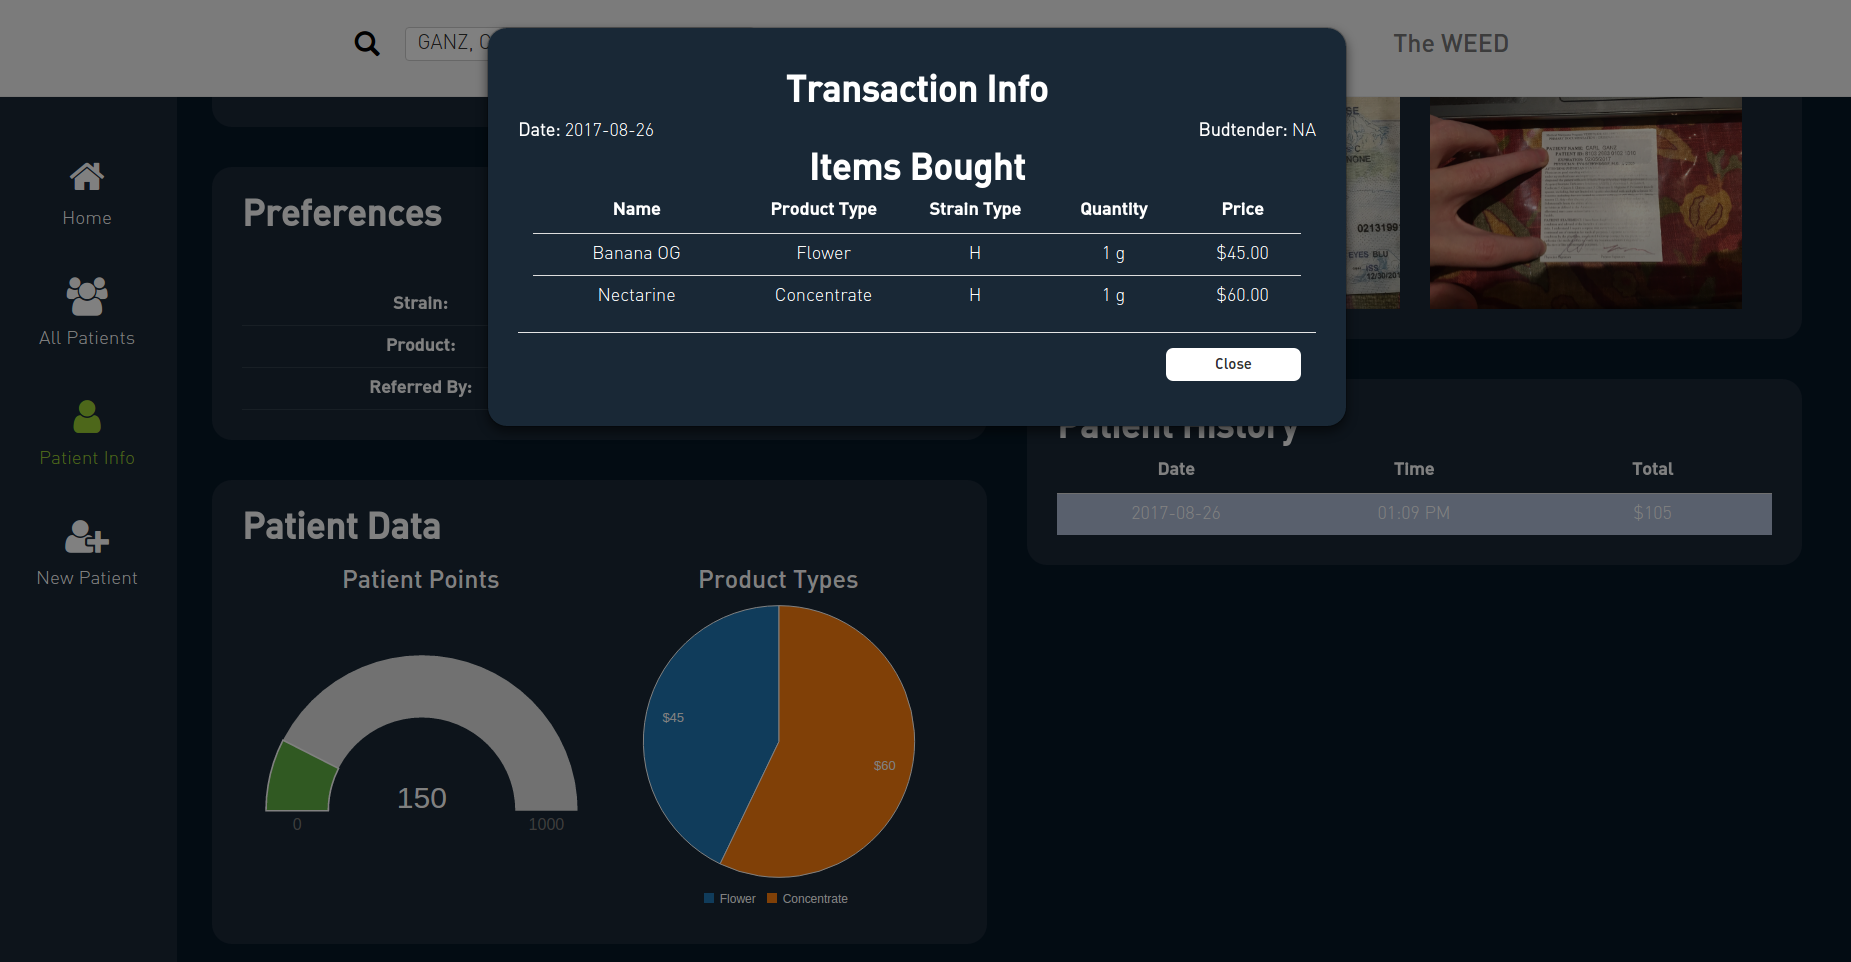
\includegraphics{images/FD5.png}
\caption{Patient History}
\end{figure}

\subsection{Updating Info}\label{updating-info}

When a patient's medical card expires they have to get a new card, and
bring that information to the dispensary. All information in the patient
info page is editable including the medical card info, and patient
images.

\begin{figure}
\centering
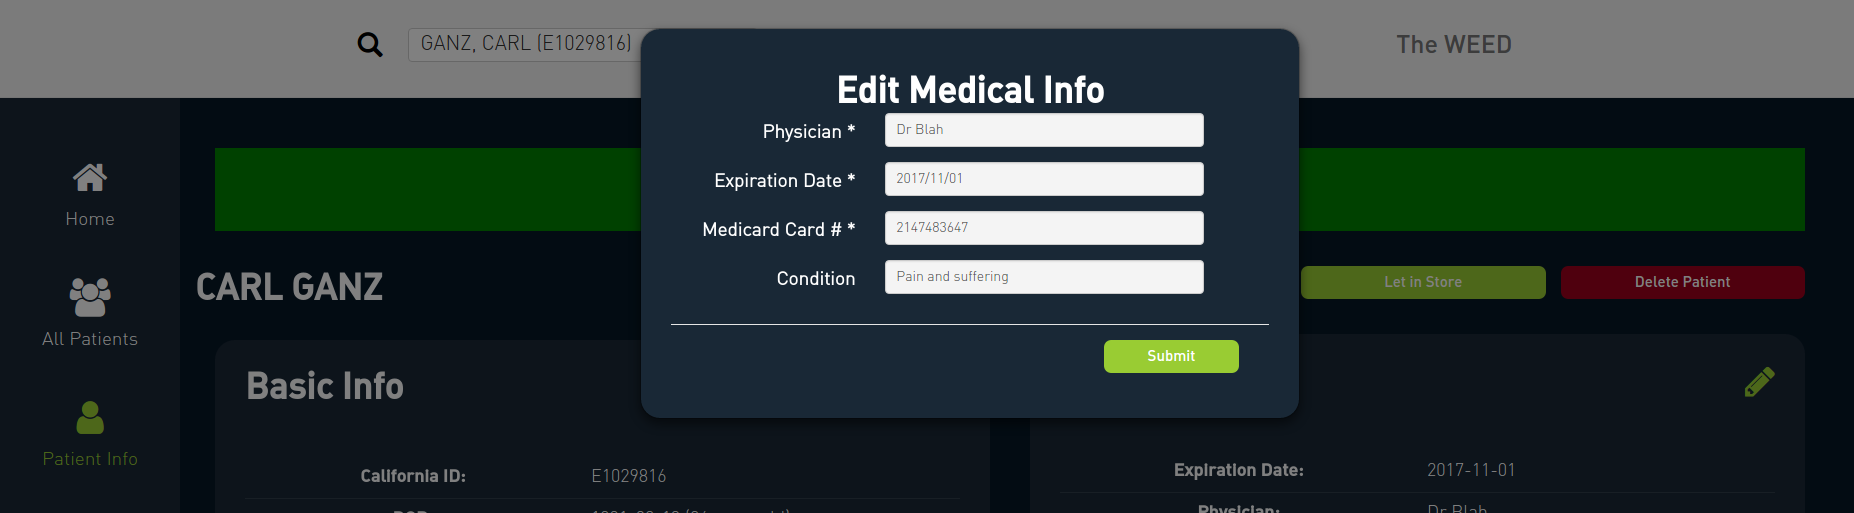
\includegraphics{images/FD6.png}
\caption{Edit Medical Info}
\end{figure}

\begin{figure}
\centering
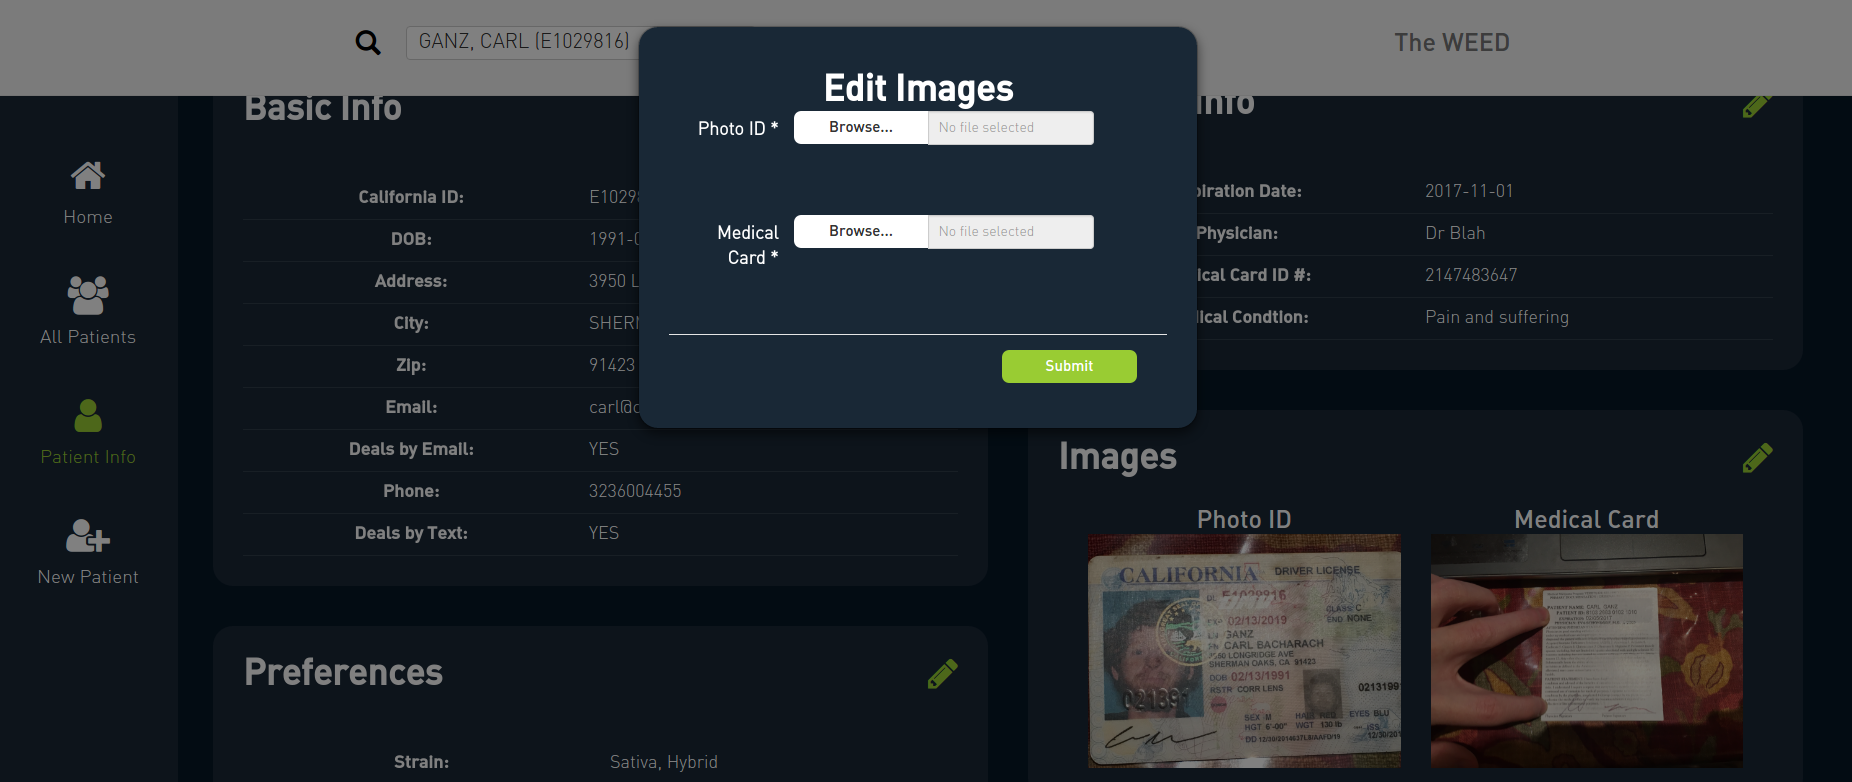
\includegraphics{images/FD7.png}
\caption{Edit Images}
\end{figure}

\section{New Patients}\label{new-patients}

For new patients, when their ID is scanned a message will appear
indicating that the patient is new. The budtender has the option to add
the new patient which initiates the patient sign-up process.

\begin{figure}
\centering
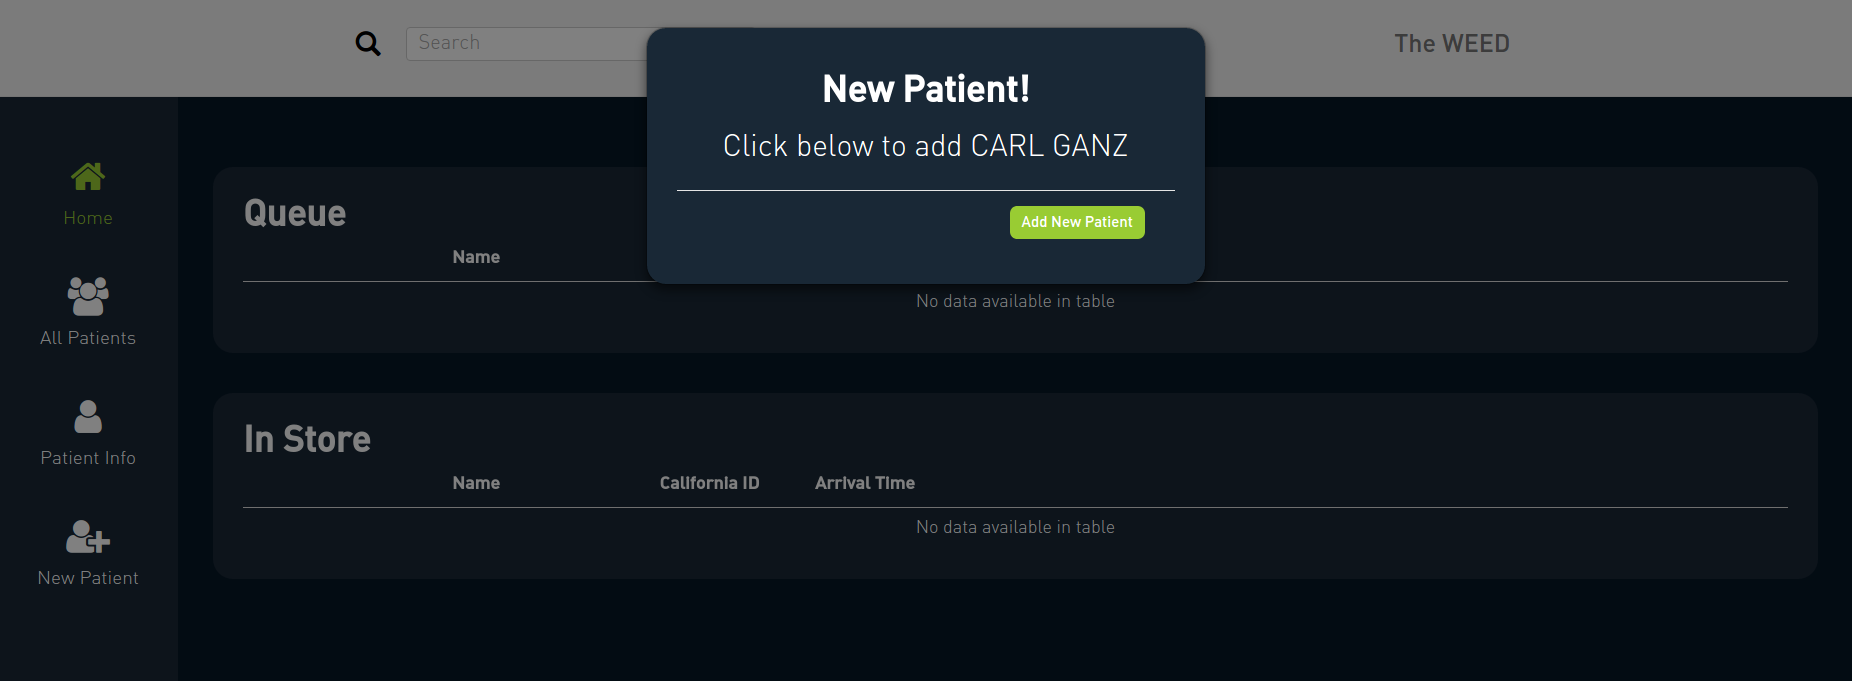
\includegraphics{images/FD10.png}
\caption{Add New Patient Screen}
\end{figure}

When the patient's ID is first scanned, the information from their ID is
automatically added. The budtender uploads the patient's documents, and
enter a small amount of information from the patient's medical card,
specifically the name of their doctor, the expiration date, and the
medical card ID number.

\begin{figure}
\centering
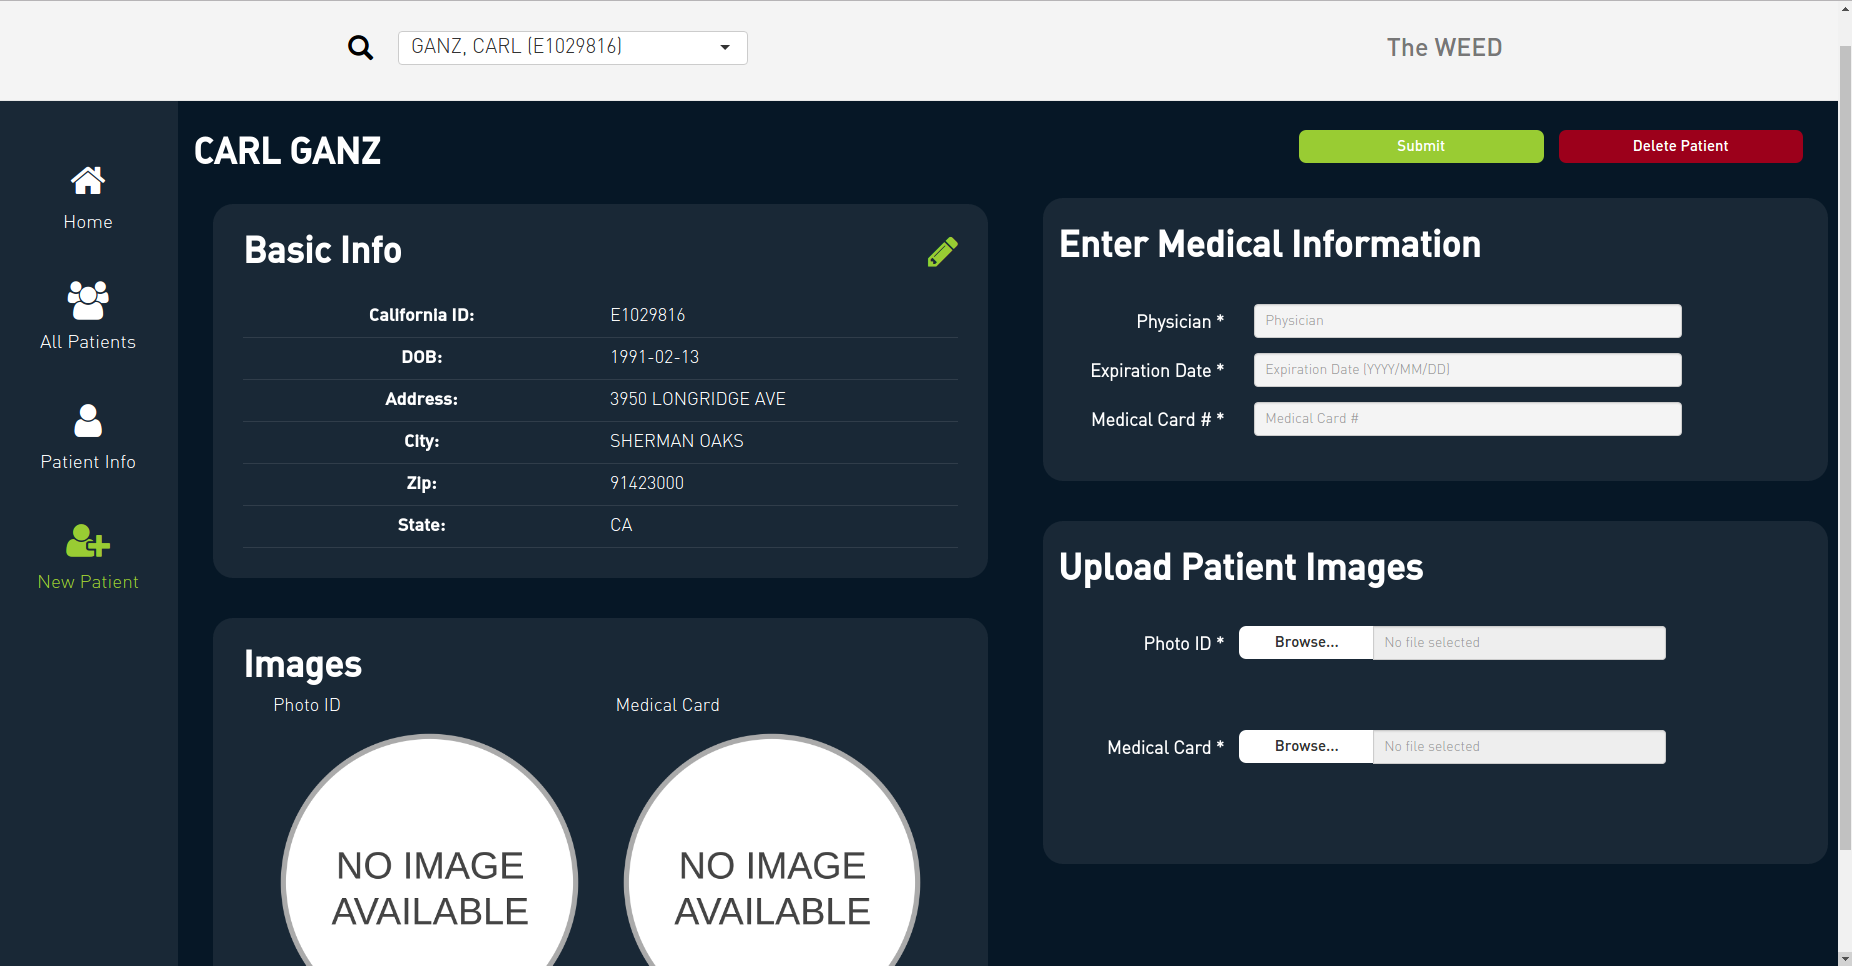
\includegraphics{images/FD11.png}
\caption{Empty New Patient Form}
\end{figure}

\begin{figure}
\centering
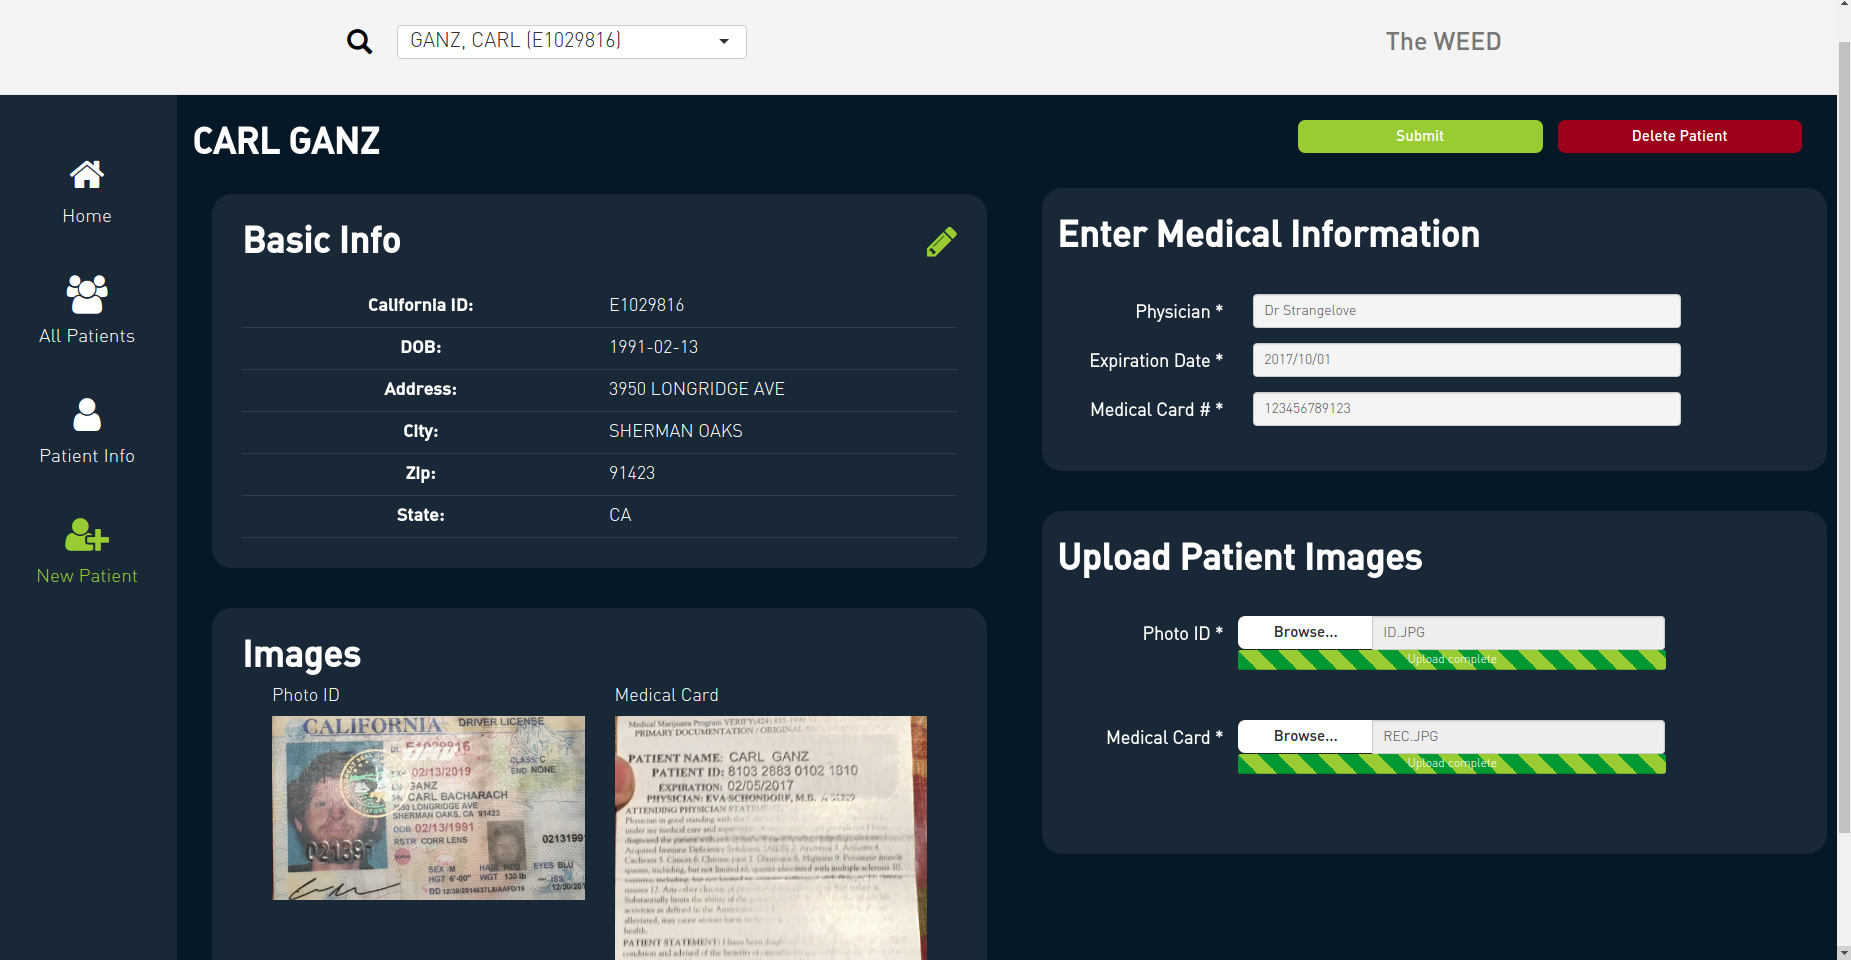
\includegraphics{images/FD9.png}
\caption{Completed New Patient Form}
\end{figure}

While the budtender enters this information, the patient is presented
with an iPad (or other tablet or computer) where they enter their
information into the Signup application discussed below.

\subsection{Signup}\label{signup}

The Signup application works in conjunction with the Frontdesk app to
let new patients quickly join a dispensary. When a new patient's ID is
scanned they are added to the database, but their profile is incomplete.
The budtender must input some information (discussed above), and the
patient must complete the signup form (and sign the patient agreement),
before they can enter the store. The first page of the signup form
contains an input where the budtender can select the incomplete profile
of the new patient.

\begin{figure}
\centering
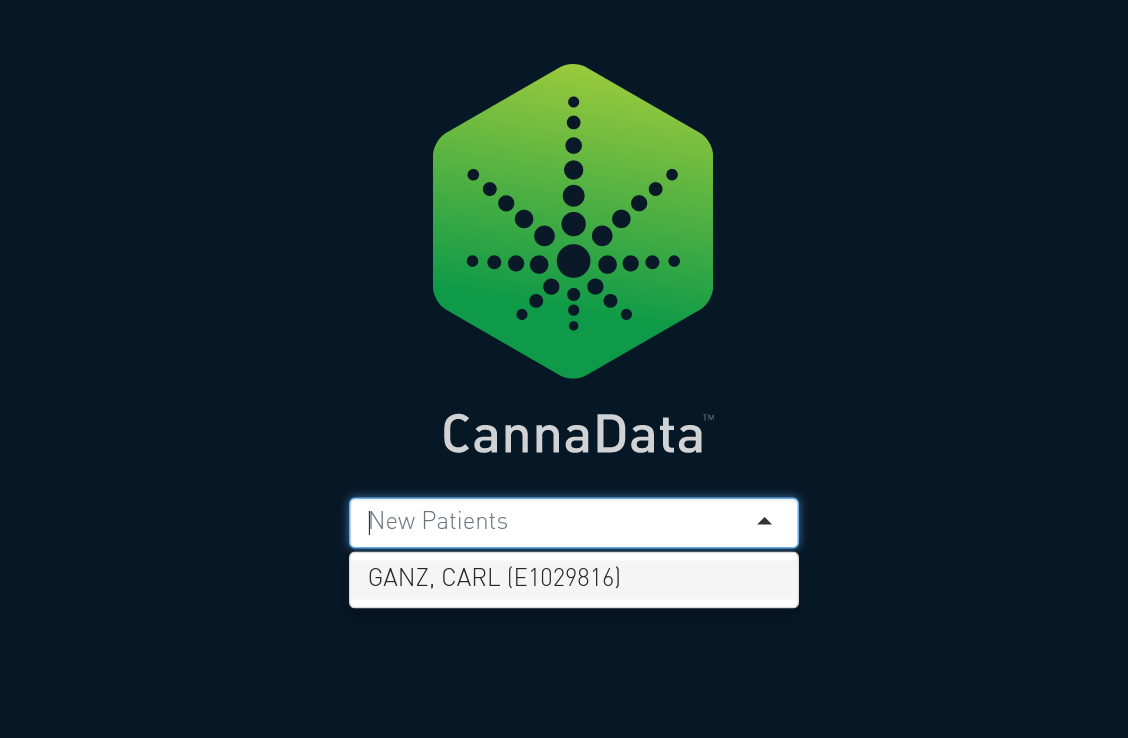
\includegraphics{images/S1.png}
\caption{Select A New Patient}
\end{figure}

Once the incomplete profile is selected the budtender would hand the
iPad over to the new patient who would fill out the rest of the form.
The first page of the signup form is automatically filled in based on
the information on the patient's driver's license.

\begin{figure}
\centering
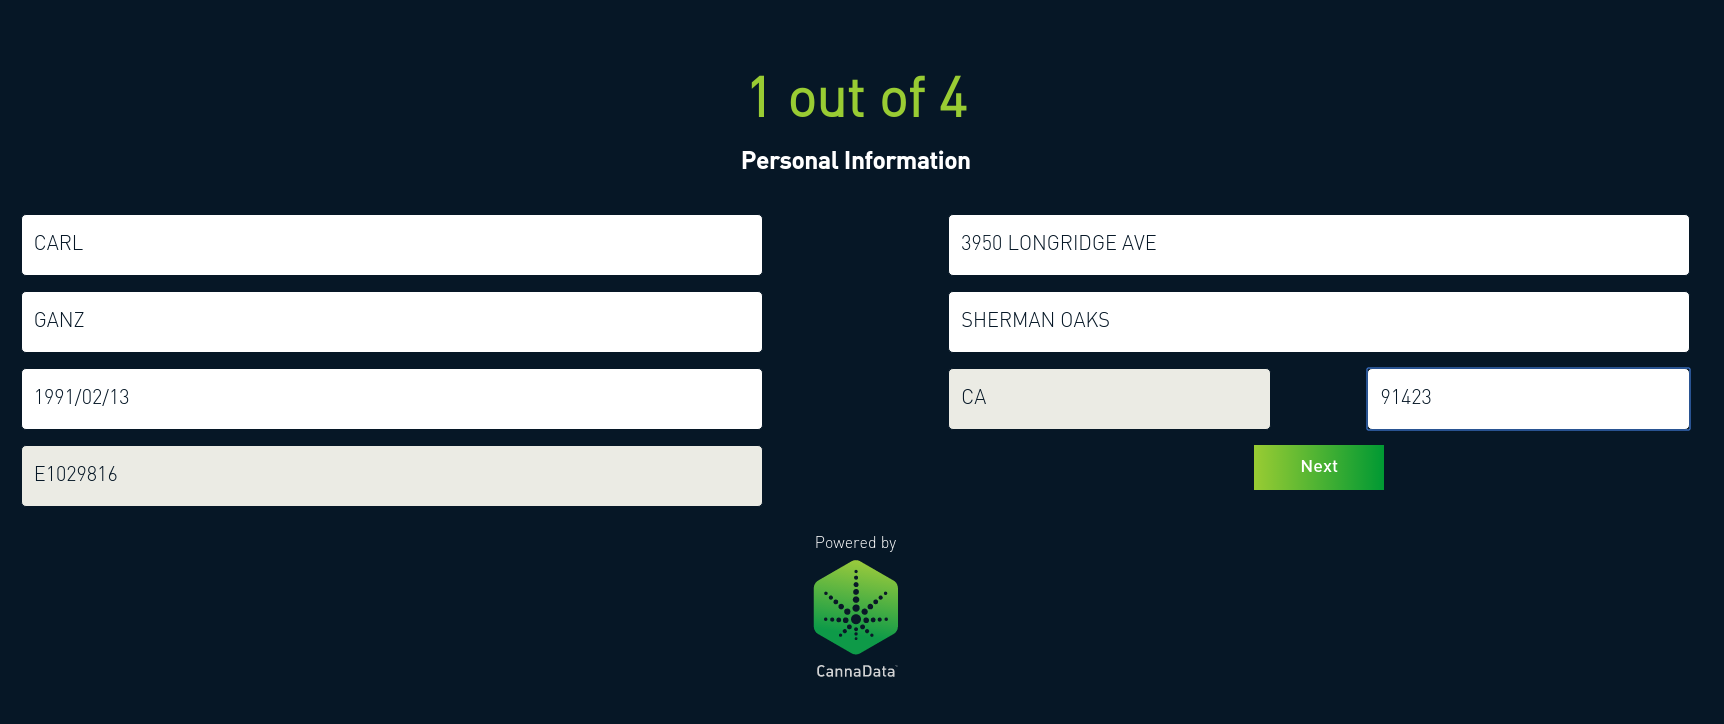
\includegraphics{images/S2.png}
\caption{Autofilled Basic Info}
\end{figure}

There are three additional pages where the patient fills in their
contact info, and preferences.

\begin{figure}
\centering
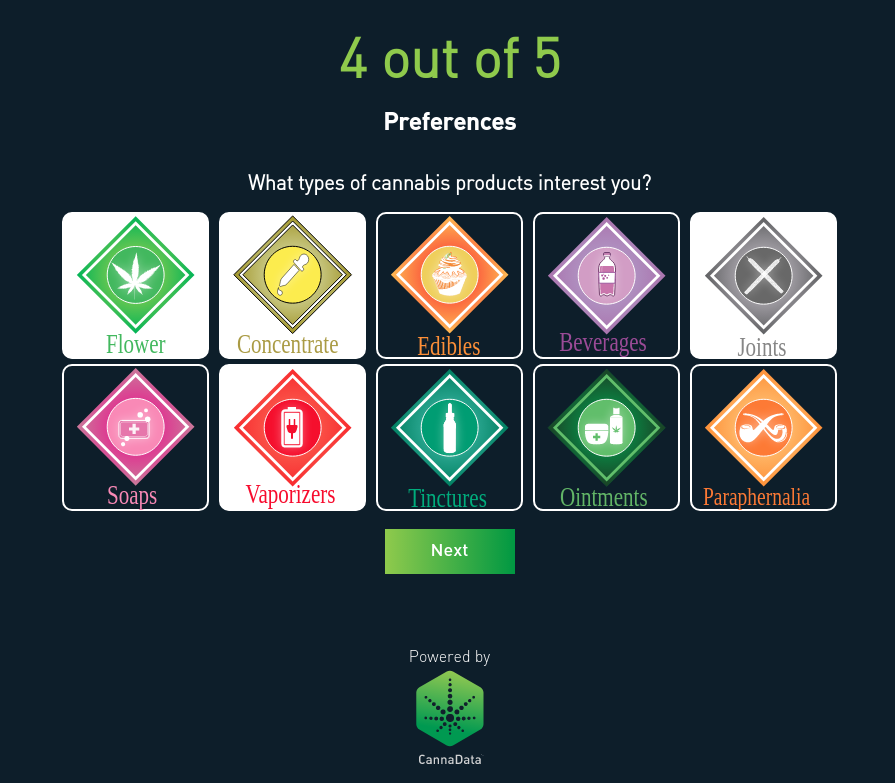
\includegraphics{images/S3.png}
\caption{Preference Info}
\end{figure}

\textbf{(NOTE TO NAYELI: I think the patient preference input is an area
where we can be creative. In liue of the plain old checkboxes we could
use cool icons representing flower, concentrate, edibles, etc.)}

After the patient completes the form they are automatically sent to a
page where they digitally sign the new patient agreement contract. This
makes the signup process completely paperless.

\chapter{Inventory}\label{inventory}

The Inventory Management application provides facilities for:

\begin{itemize}
\item
  Adding new inventory and new wholesalers
\item
  Viewing the performance of past products and wholesalers
\item
  Checking quantities of current stock
\item
  Updating/editing information about existing products
\item
  Print labels/barcodes for inventory
\end{itemize}

\section{New Inventory}\label{new-inventory}

The new inventory page allows you to enter new shipments of inventory
into your database. Digitally managing inventory doesn't just make it
easier to keep track of products, but it also simplifies the record
keeping process required for taxes, and other regulations.

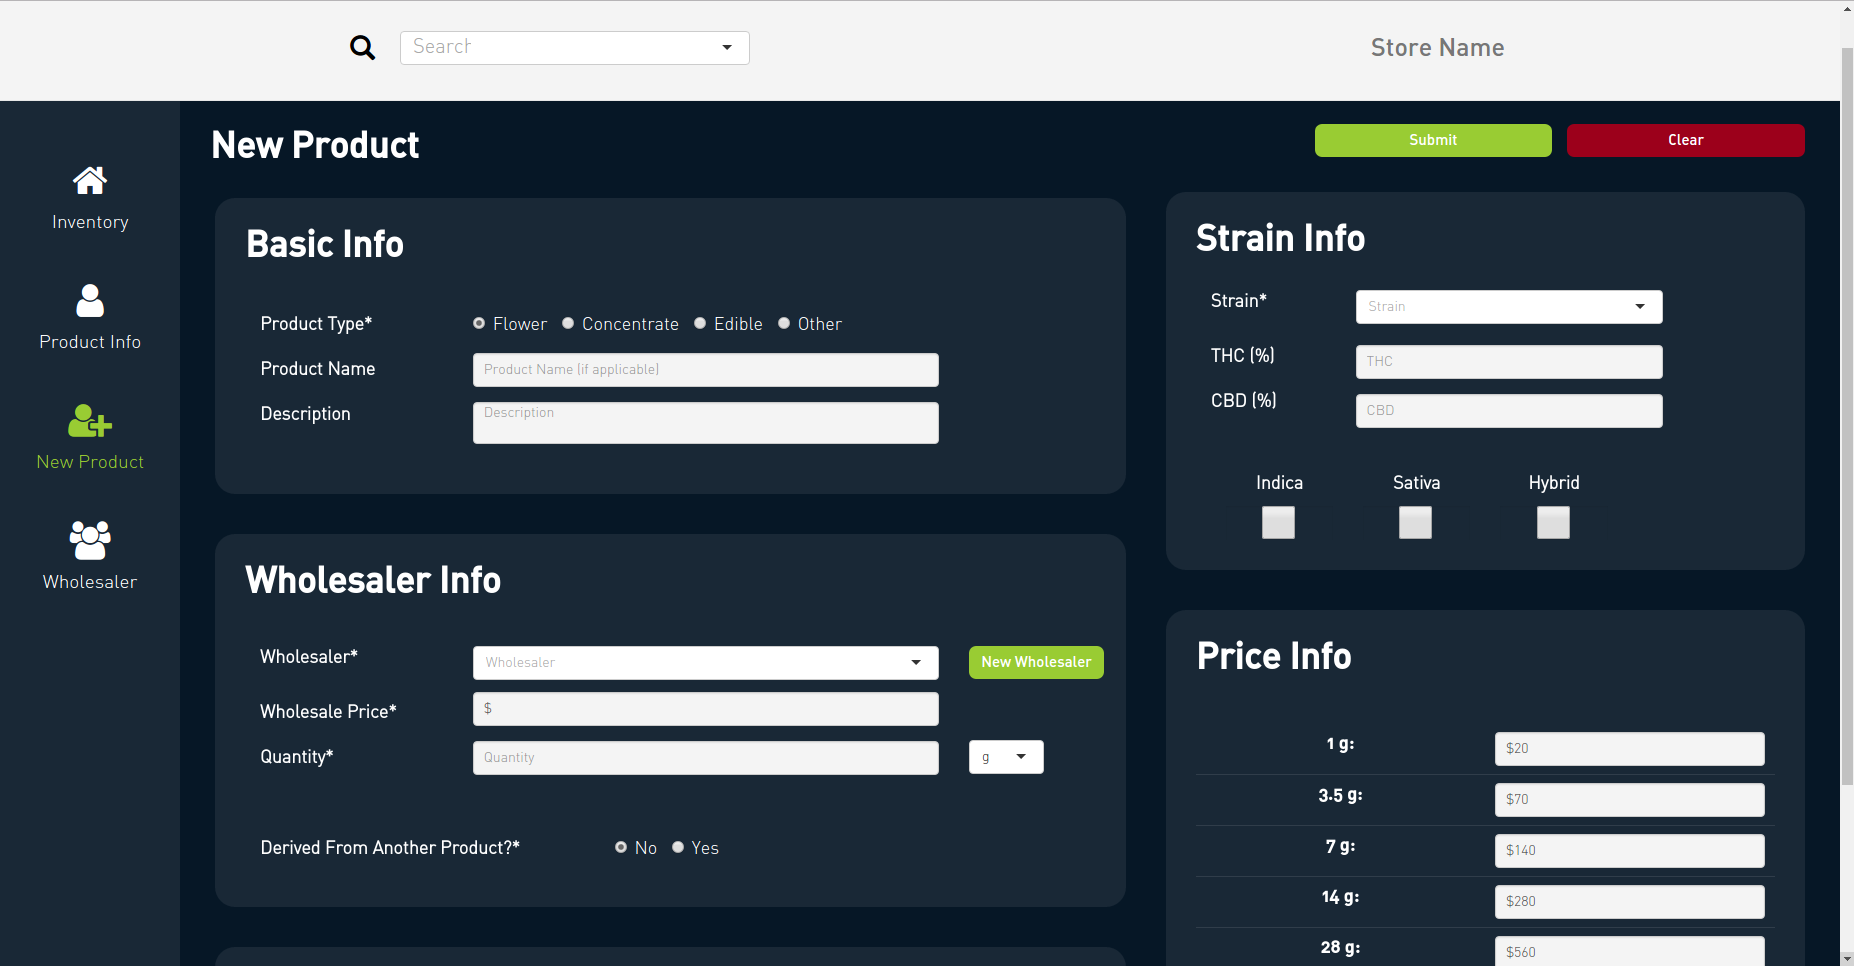
\includegraphics{images/I1.png} 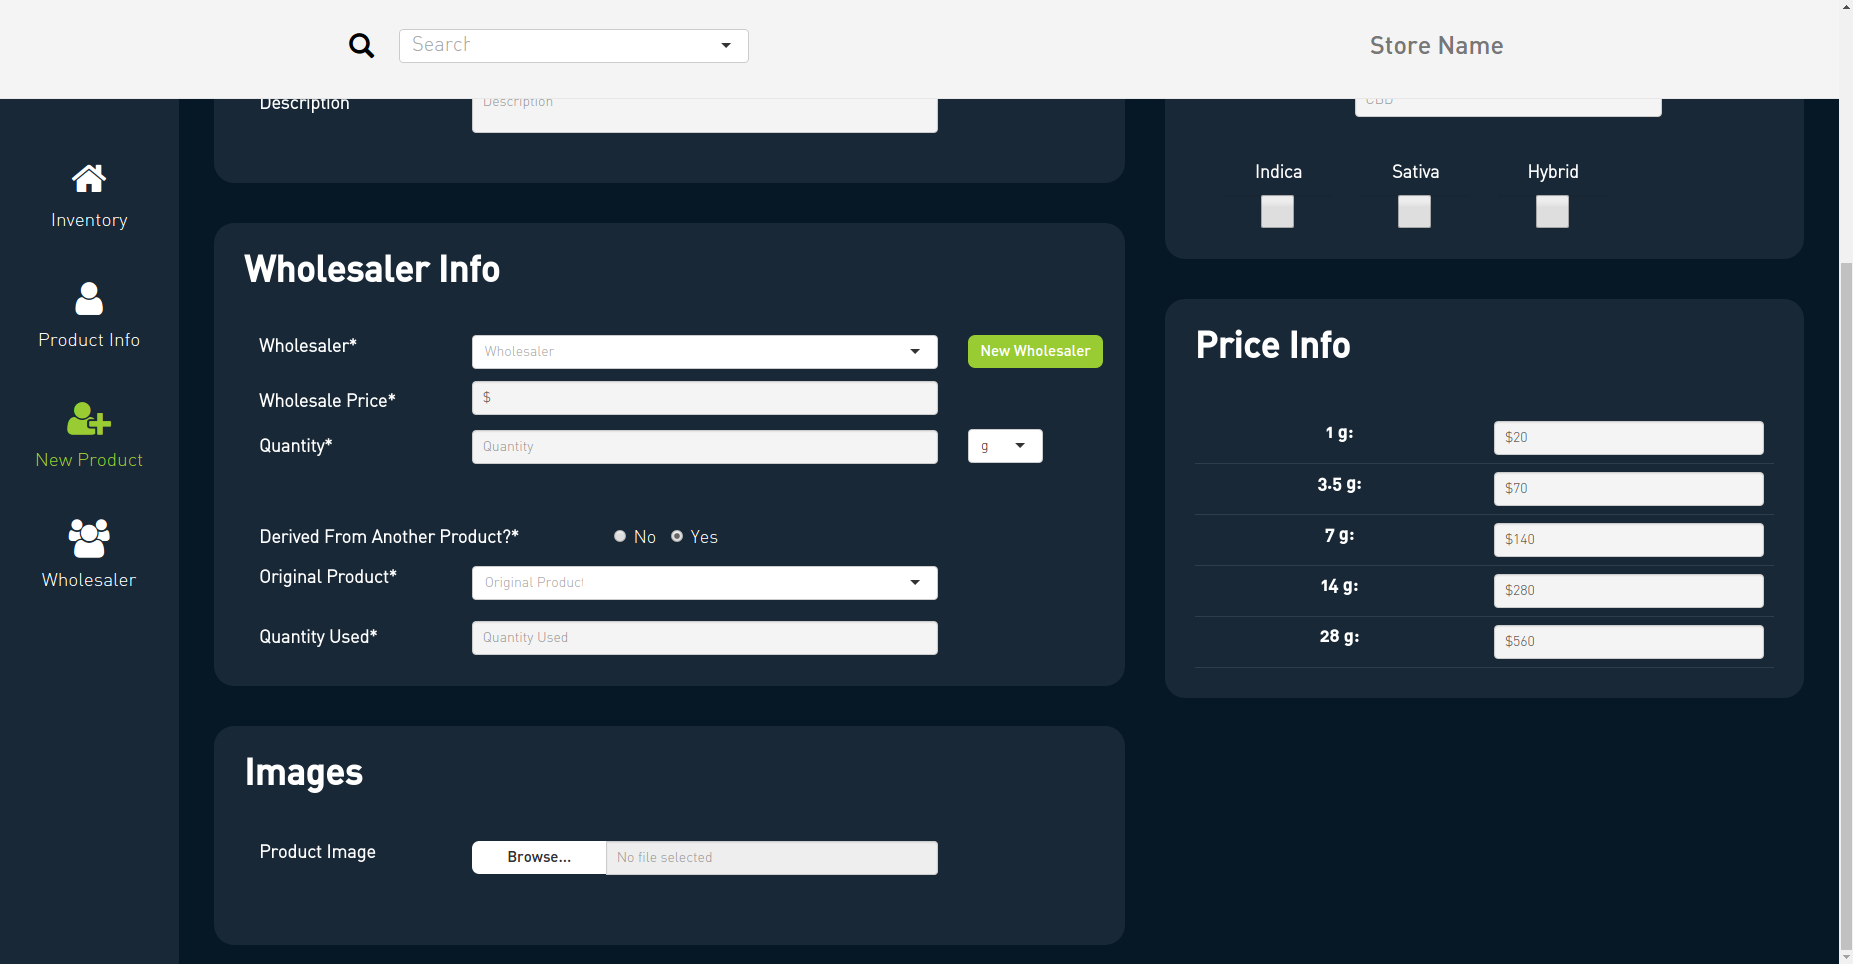
\includegraphics{images/I2.png}

There are several required fields in the new inventory form:

\begin{itemize}
\item
  Product Type (i.e.~flower vs concentrate vs edible etc.)
\item
  Strain (No strain is an option, but must be explicitely selected)
\item
  Wholesaler
\item
  Wholesale price
\item
  Quantity
\item
  Price
\end{itemize}

There are also several optional inputs, and inputs that are only
required sometimes:

\begin{itemize}
\item
  Product Name (required if no strain selected)
\item
  Description
\item
  THC \& CBD levels
\item
  Whether product is Indica/Sativa/Hybrid
\item
  Image
\item
  Source product and quantity (i.e.~if you take 50 grams of Banana OG
  and make 75 joints, when you enter the 75 joints you would also want
  to remove the 50 grams of Banana OG that the joints are derived from)
\end{itemize}

\subsection{Pricing}\label{pricing}

The price input contains default values based on the product type.
Whenever a value in the price input is updated, the rows below the
changed value, representing the price for larger quantities, are updated
to be consistent with the new value. For example, the default price for
concentrates is \$30 per half gram. This rate is used for higher
quantities so 1 gram is \$30*2=\$60, two grams is \$30*4=\$120, etc. We
can update the price for two grams to \$100, which translates to \$50
per gram. Now all quantities above two grams are priced at the \$50 per
gram rate, while all quantities below two grams retain the \$30 per half
gram (\$60 per gram) rate.

\begin{figure}
\centering
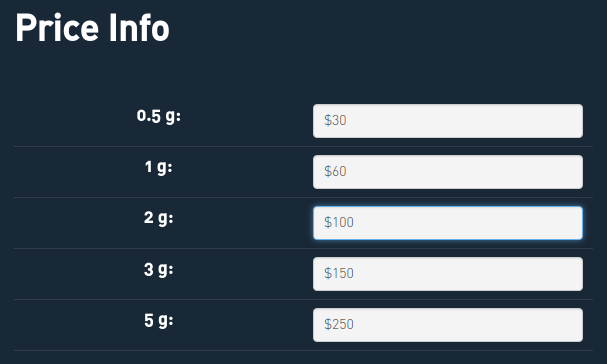
\includegraphics{images/I3.png}
\caption{Price Input with 2 g level manually set to \$100}
\end{figure}

\section{Past Products}\label{past-products}

Details about existing and past products are easily accessible. You can
search for any past inventory and all wholesalers in the search box at
the top. You can also view current inventory in the current inventory
table.

\begin{figure}
\centering
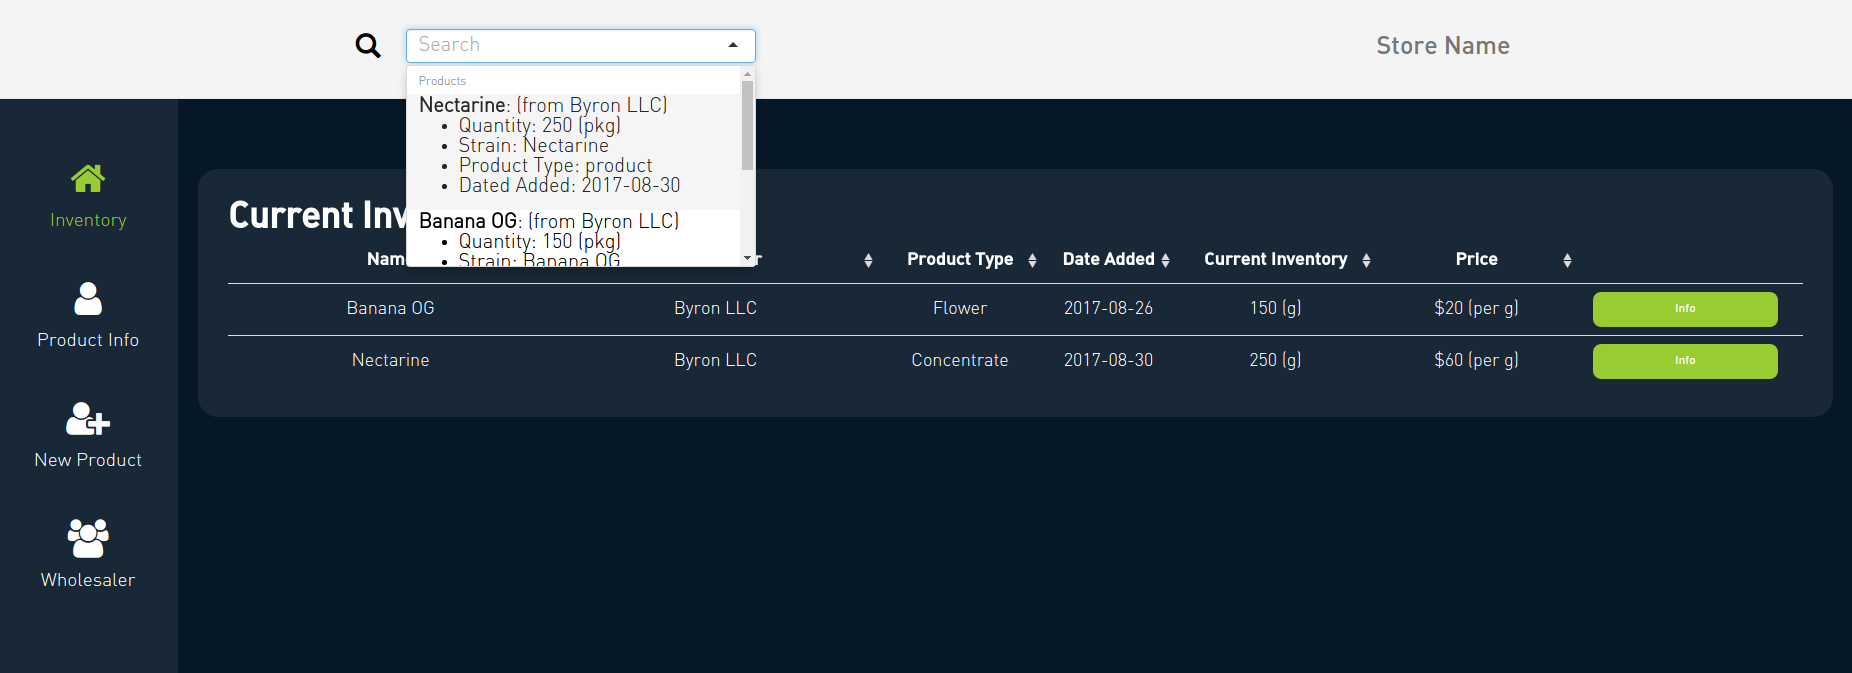
\includegraphics{images/I4.png}
\caption{Current Inventory Table}
\end{figure}

When you select an item you are taken to the product information page.
This includes a variety of tables regarding the specific product with
the option to edit. Buttons at the top allow to quickly add more
inventory and print barcodes for the product.

\begin{figure}
\centering
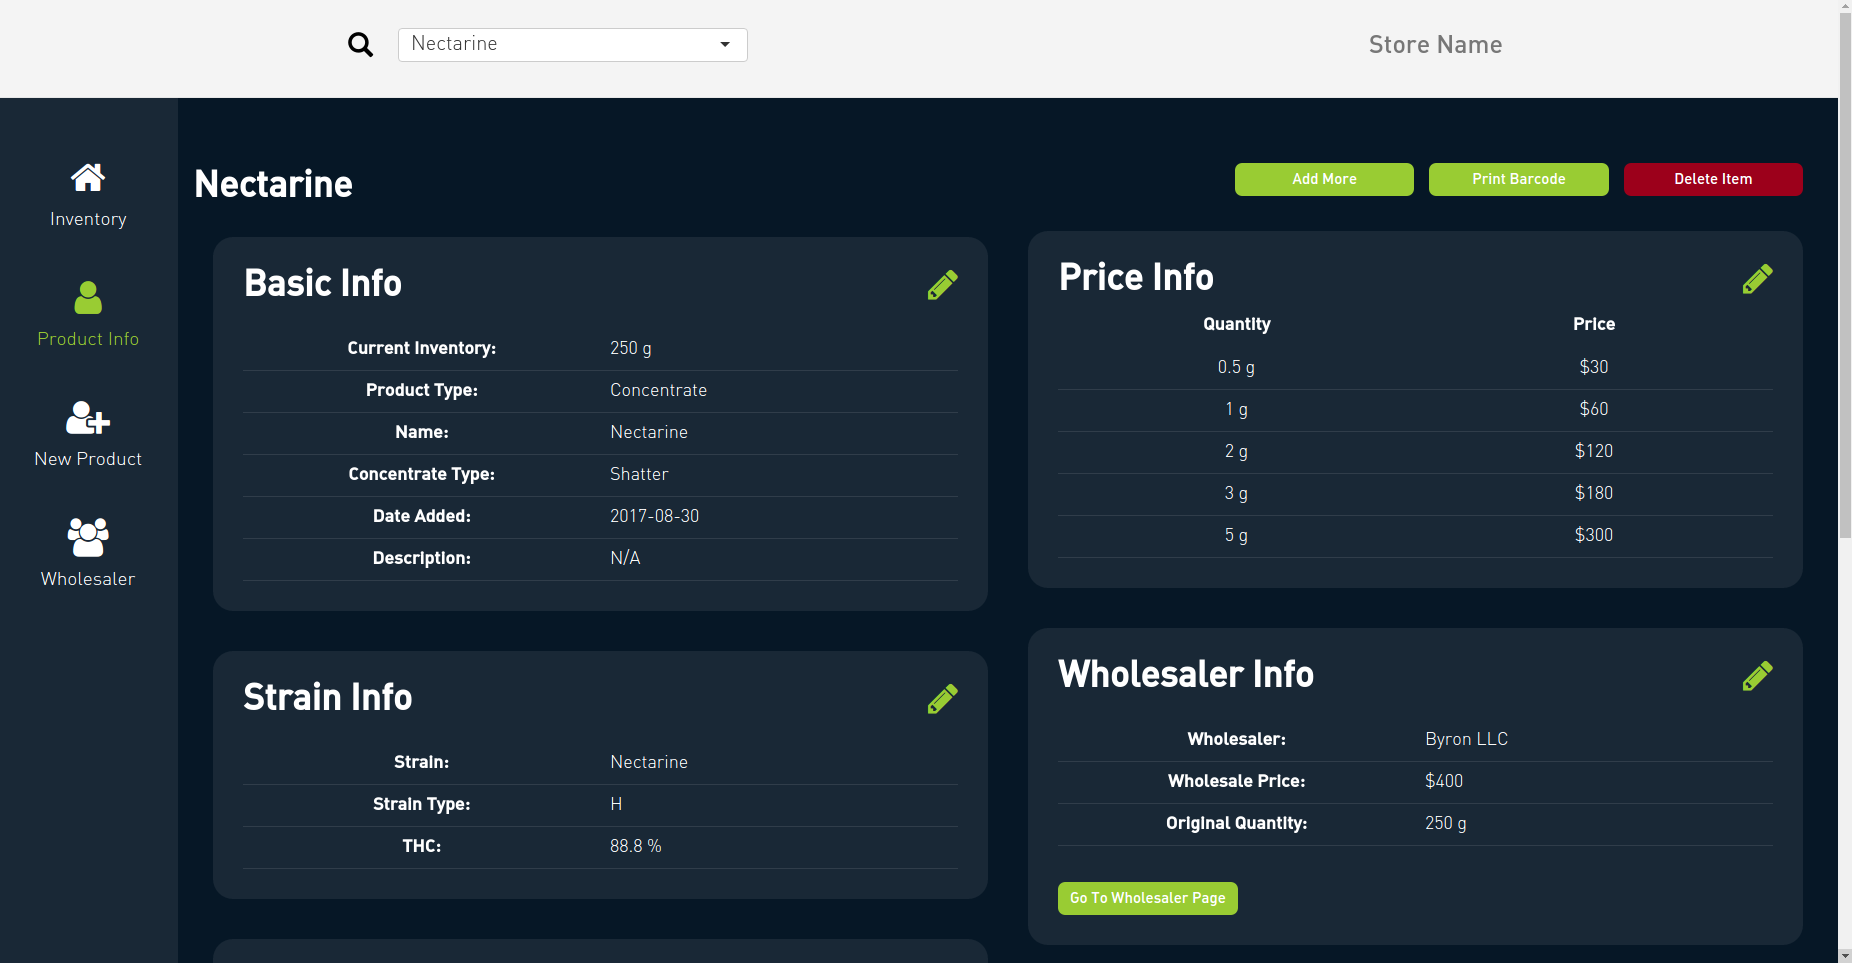
\includegraphics{images/I5.png}
\caption{Current Inventory Table}
\end{figure}

Basic analytics are provided so you can quickly see how the product is
performing. Daily sales are charted, and average daily profit is rated
against other similar products.

\begin{figure}
\centering
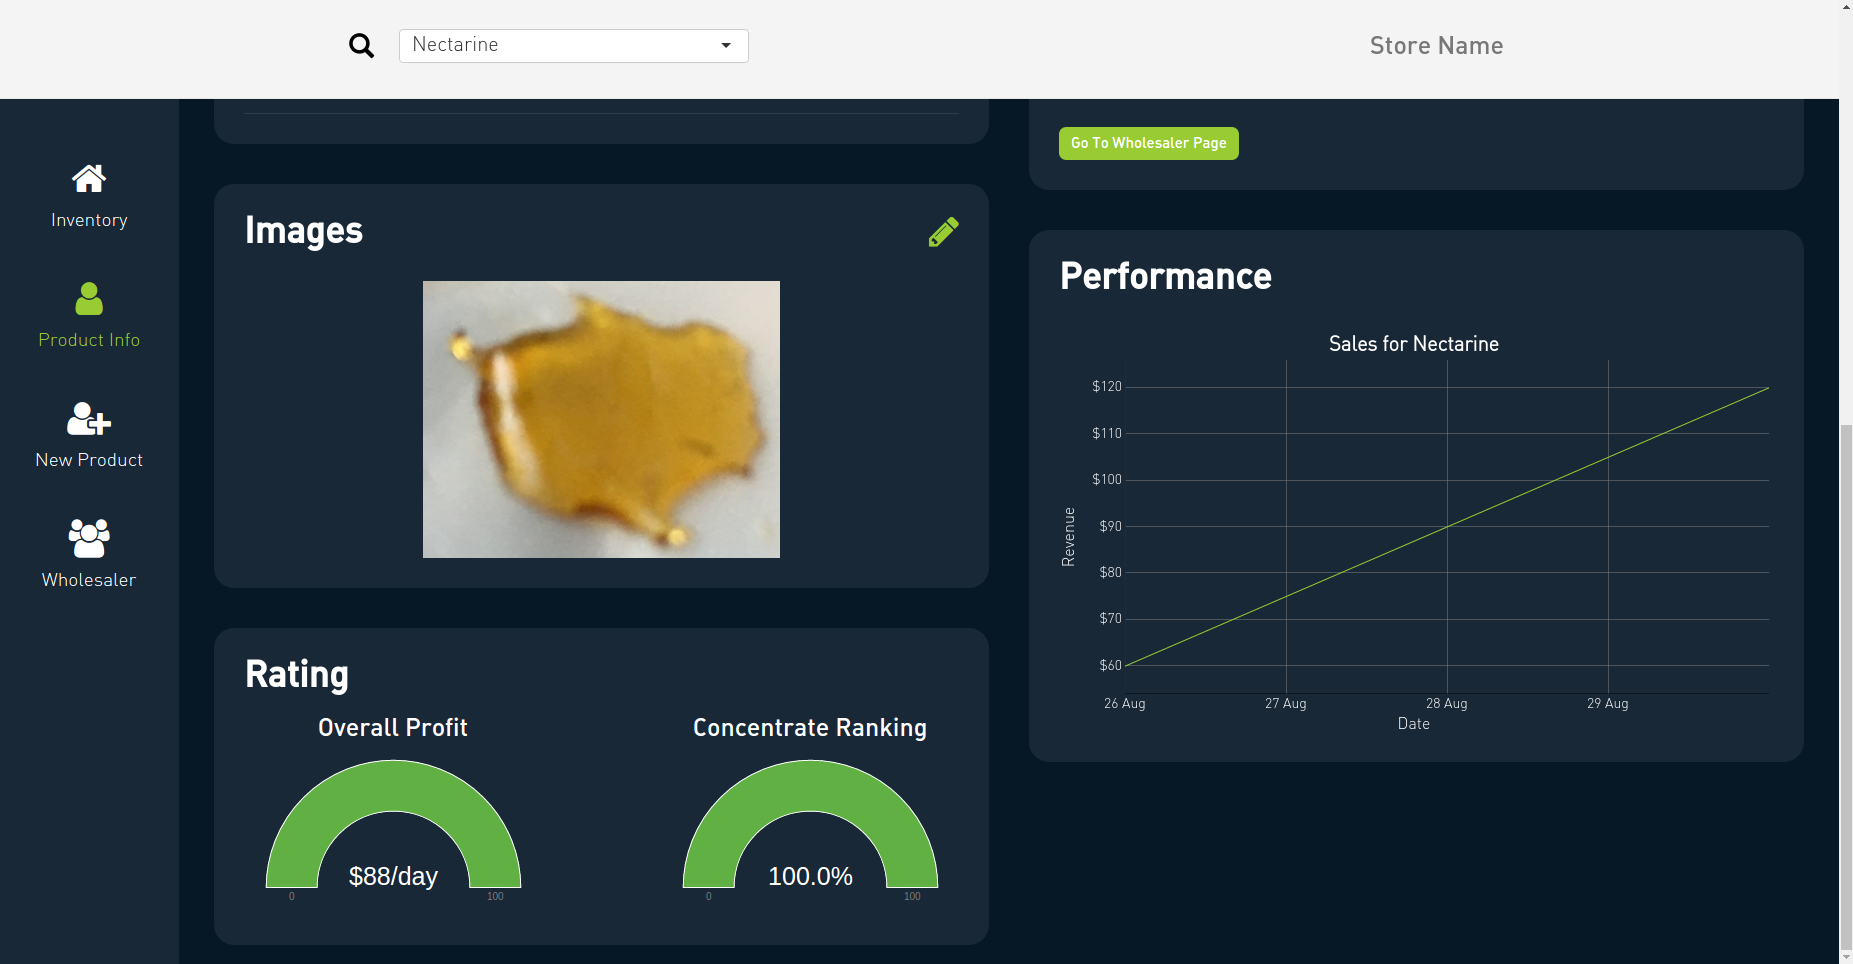
\includegraphics{images/I6.png}
\caption{Current Inventory Table}
\end{figure}

\section{Wholesaler}\label{wholesaler}

You can also view information about specific wholesalers. When you
select an item the item's wholesaler is available in the wholesaler
page. You can also select a wholesaler in the search box at the top.

\begin{figure}
\centering
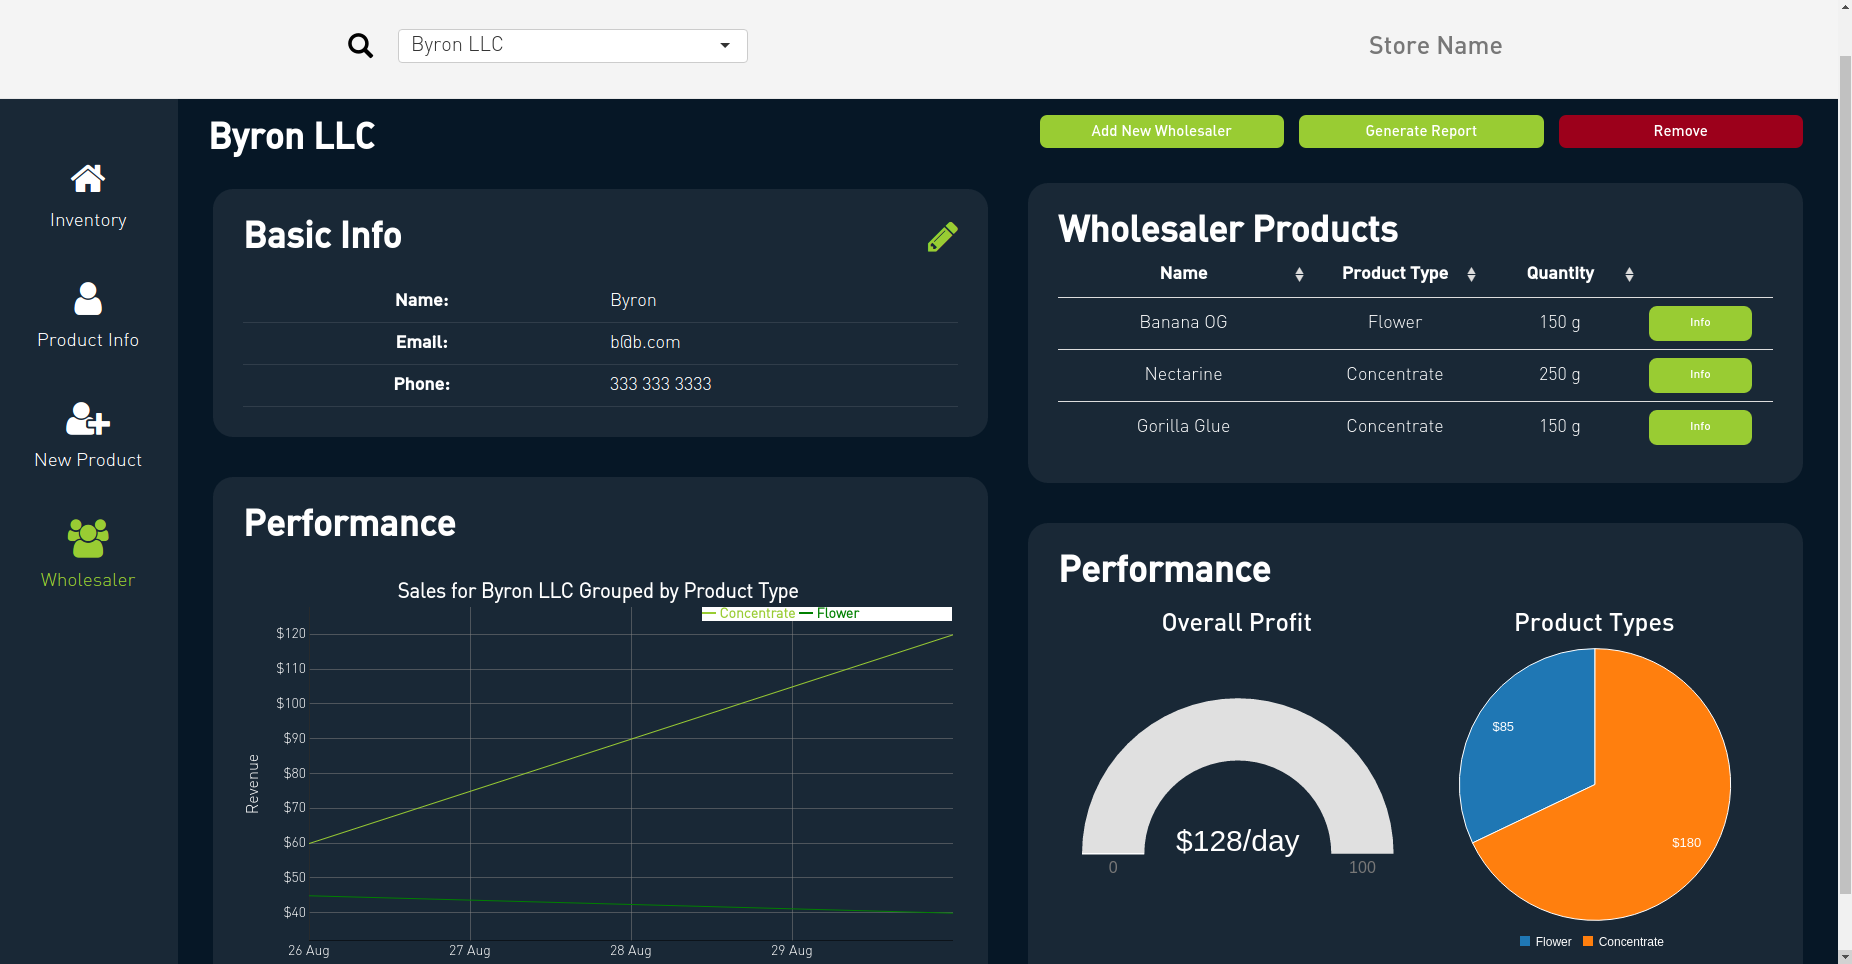
\includegraphics{images/I7.png}
\caption{Current Inventory Table}
\end{figure}

Analytics about the wholesaler including daily sales, average daily
profit, and product type.

\chapter{Connect}\label{connect}

Many dispensaries try to encourage patients to come to their store with
coupons, and targeted messages. The Connect Application provides
facilities for:

\begin{itemize}
\item
  Creating coupons/deals
\item
  Reaching out to patients via text, or email
\end{itemize}

\section{Coupons}\label{coupons}

\subsection{New Coupons}\label{new-coupons}

The required information for a new coupon is:

\begin{itemize}
\item
  A name
\item
  A discount (either a flat amount i.e. \$10, or a percentage i.e.~10\%)
\item
  A minimum (either a minimum total amount spent i.e. \$60, or a
  quantity i.e.~3.5 grams)
\item
  Which products the discount applies to. Options include:
\end{itemize}

\begin{enumerate}
\def\labelenumi{\arabic{enumi}.}
\tightlist
\item
  Total (i.e.~take 10\% off total bill)
\item
  All products of a certain type (i.e.~on Wax Wednesdays you discount
  \textbf{all} concentrates)
\item
  Specific products
\end{enumerate}

\begin{itemize}
\tightlist
\item
  Lastly you have to choose when the coupon is active
\end{itemize}

\begin{figure}
\centering
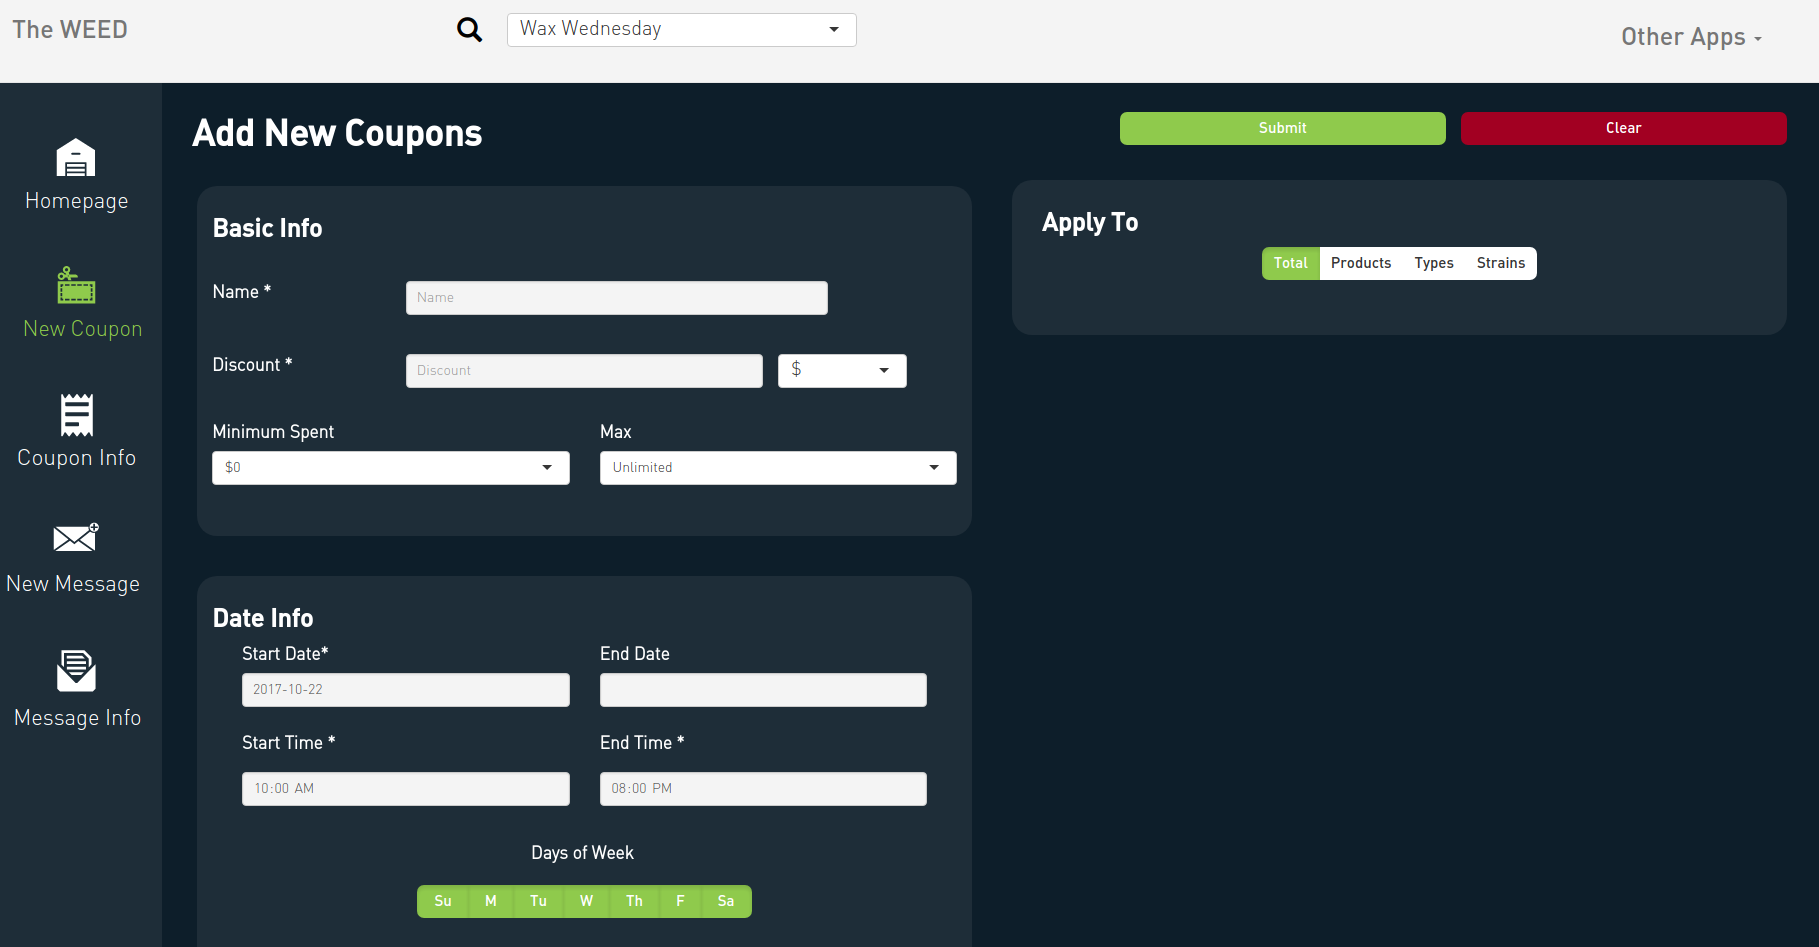
\includegraphics{images/C1.png}
\caption{Blank new coupon}
\end{figure}

\begin{figure}
\centering
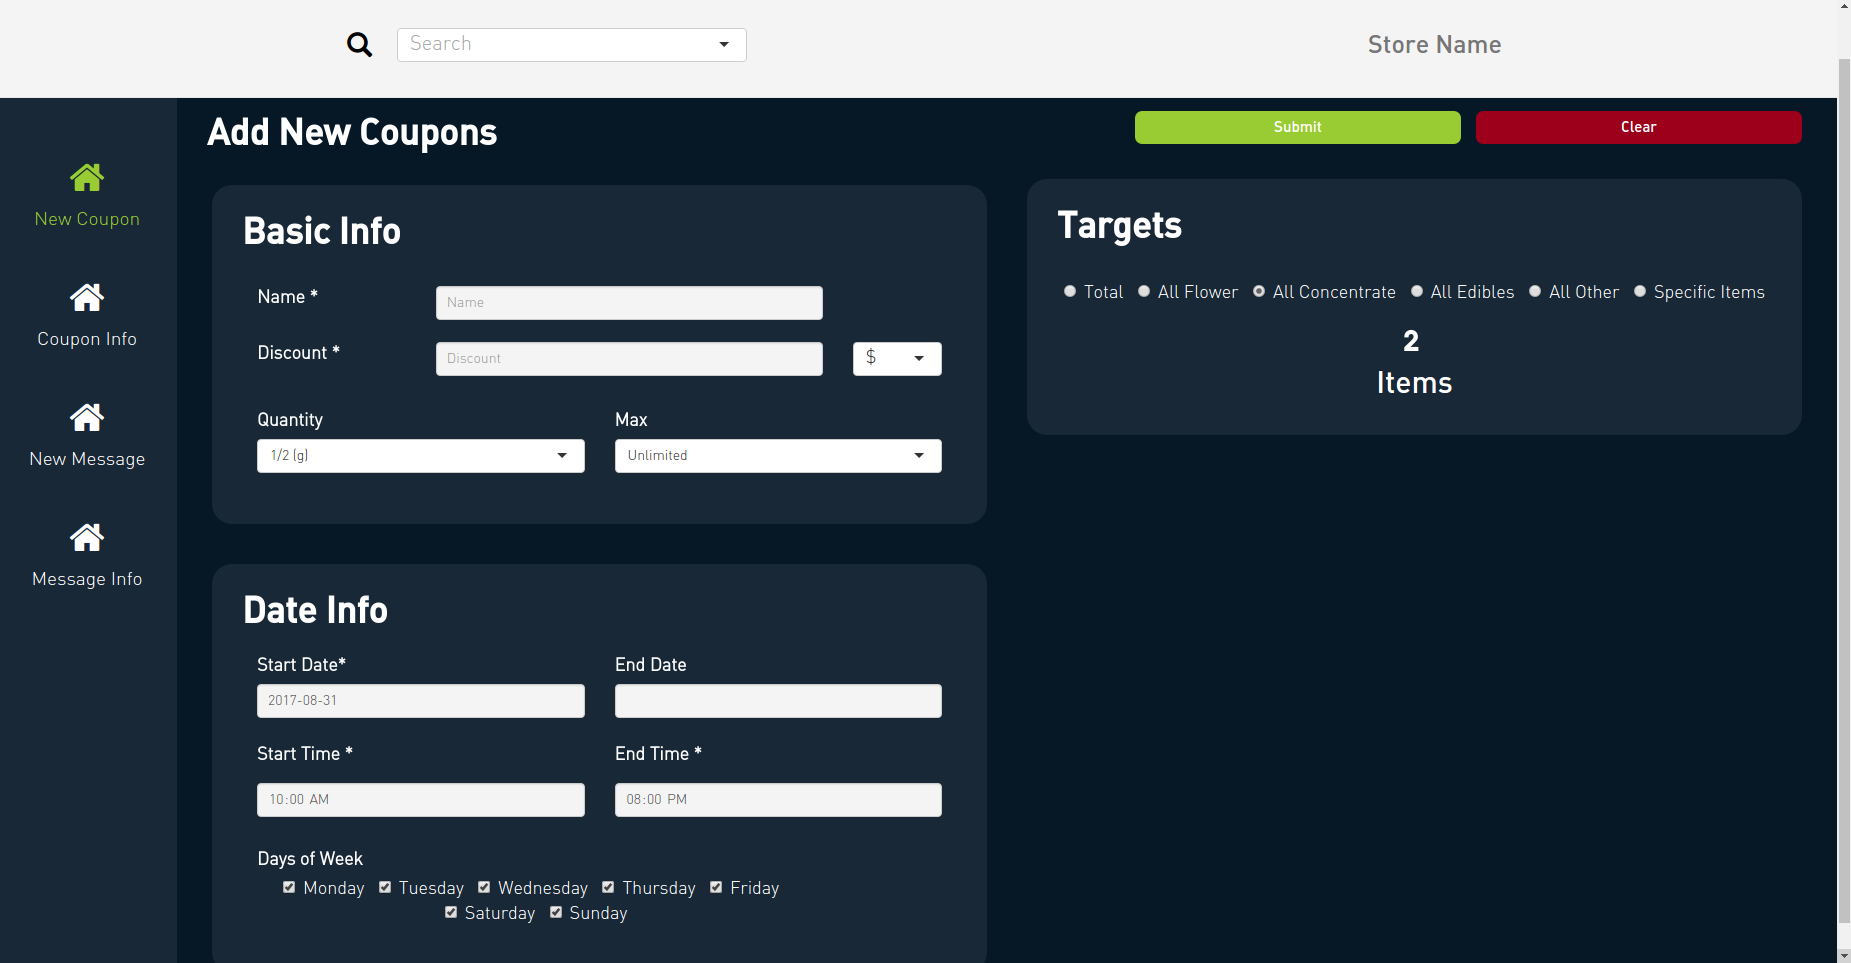
\includegraphics{images/C2.png}
\caption{Blank new coupon targeted at all concentrates}
\end{figure}

\begin{figure}
\centering
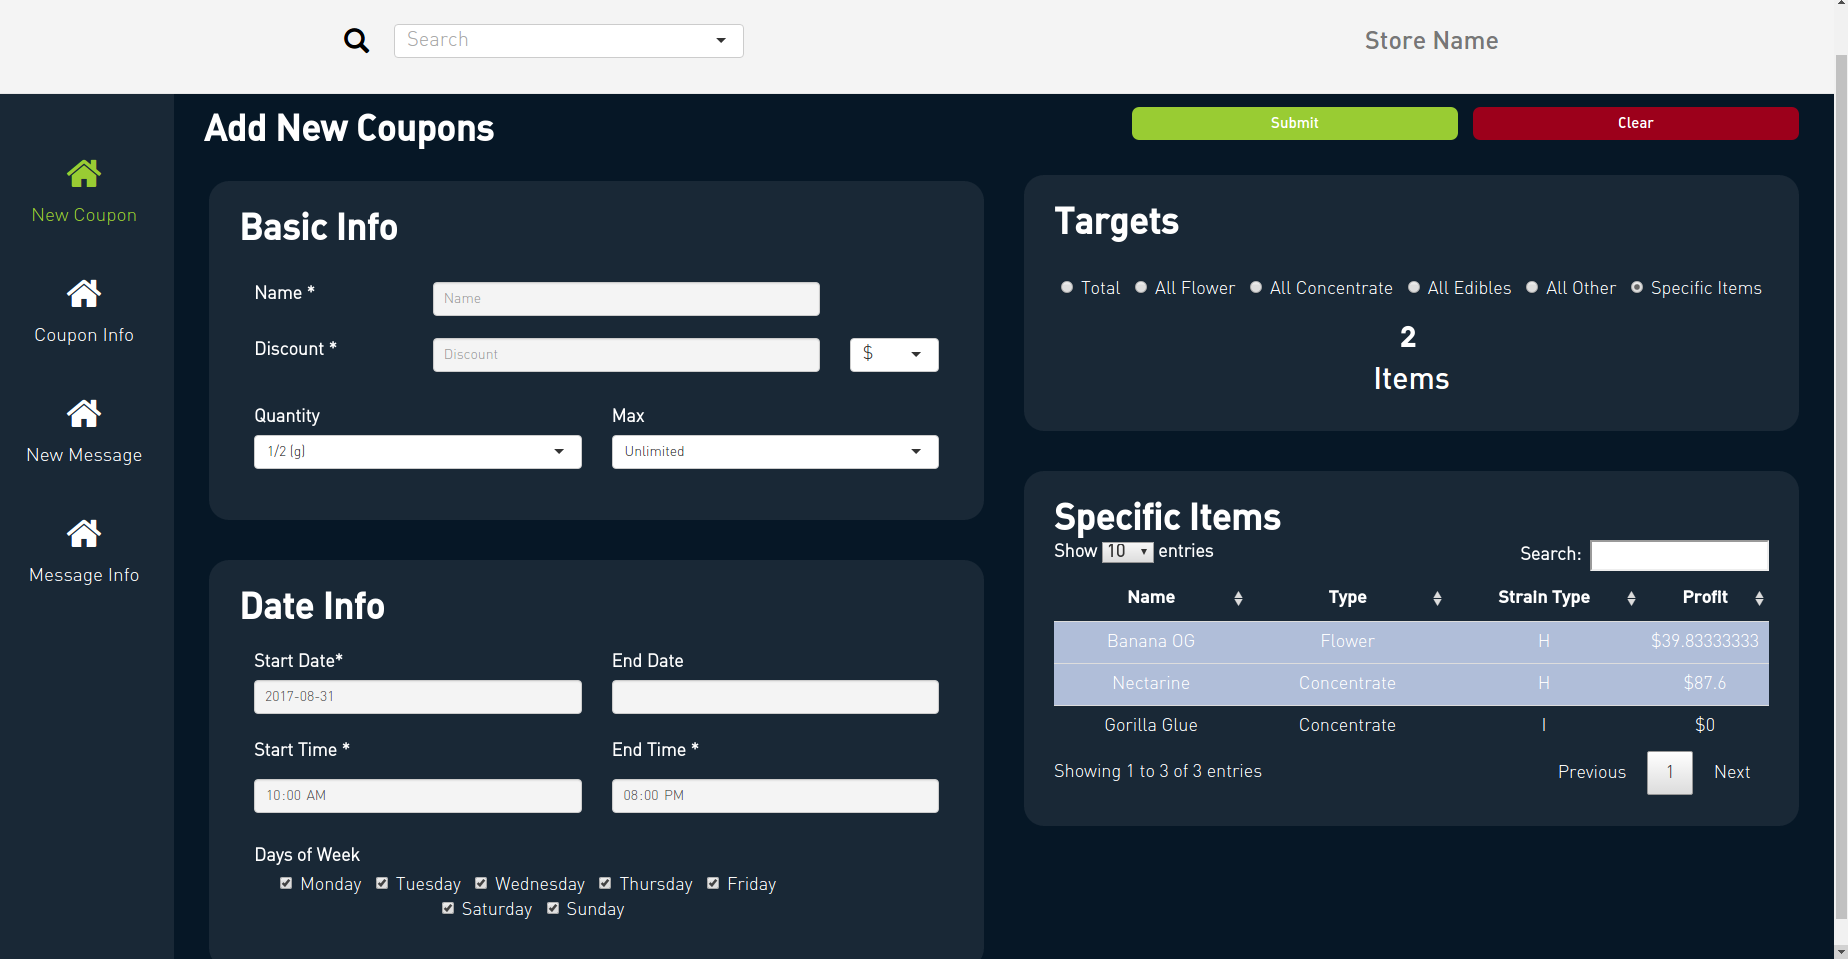
\includegraphics{images/C3.png}
\caption{Blank new coupon targeted at specific items}
\end{figure}

\textbf{(NOTE TO NAYELI: For specific items there is a problem in that
you are forced to select a single discount, and quantity for all the
specific items. It would be better if they could select different
discounts and quantities for the individual items. When you send me code
for menu I may use a version of that to recreate the specific item part.
I'd appreciate your thoughts here.)}

\subsection{Coupon Info}\label{coupon-info}

You can view information about existing coupons by selecting them in the
search box in the top. The coupon info page provides basic information
that can be edited as well as a list of current inventory that is
discounted when the coupon is active. There is a graph of daily sales
for the discounted products, which enables you to see if the coupon
created a positive bump.

\begin{figure}
\centering
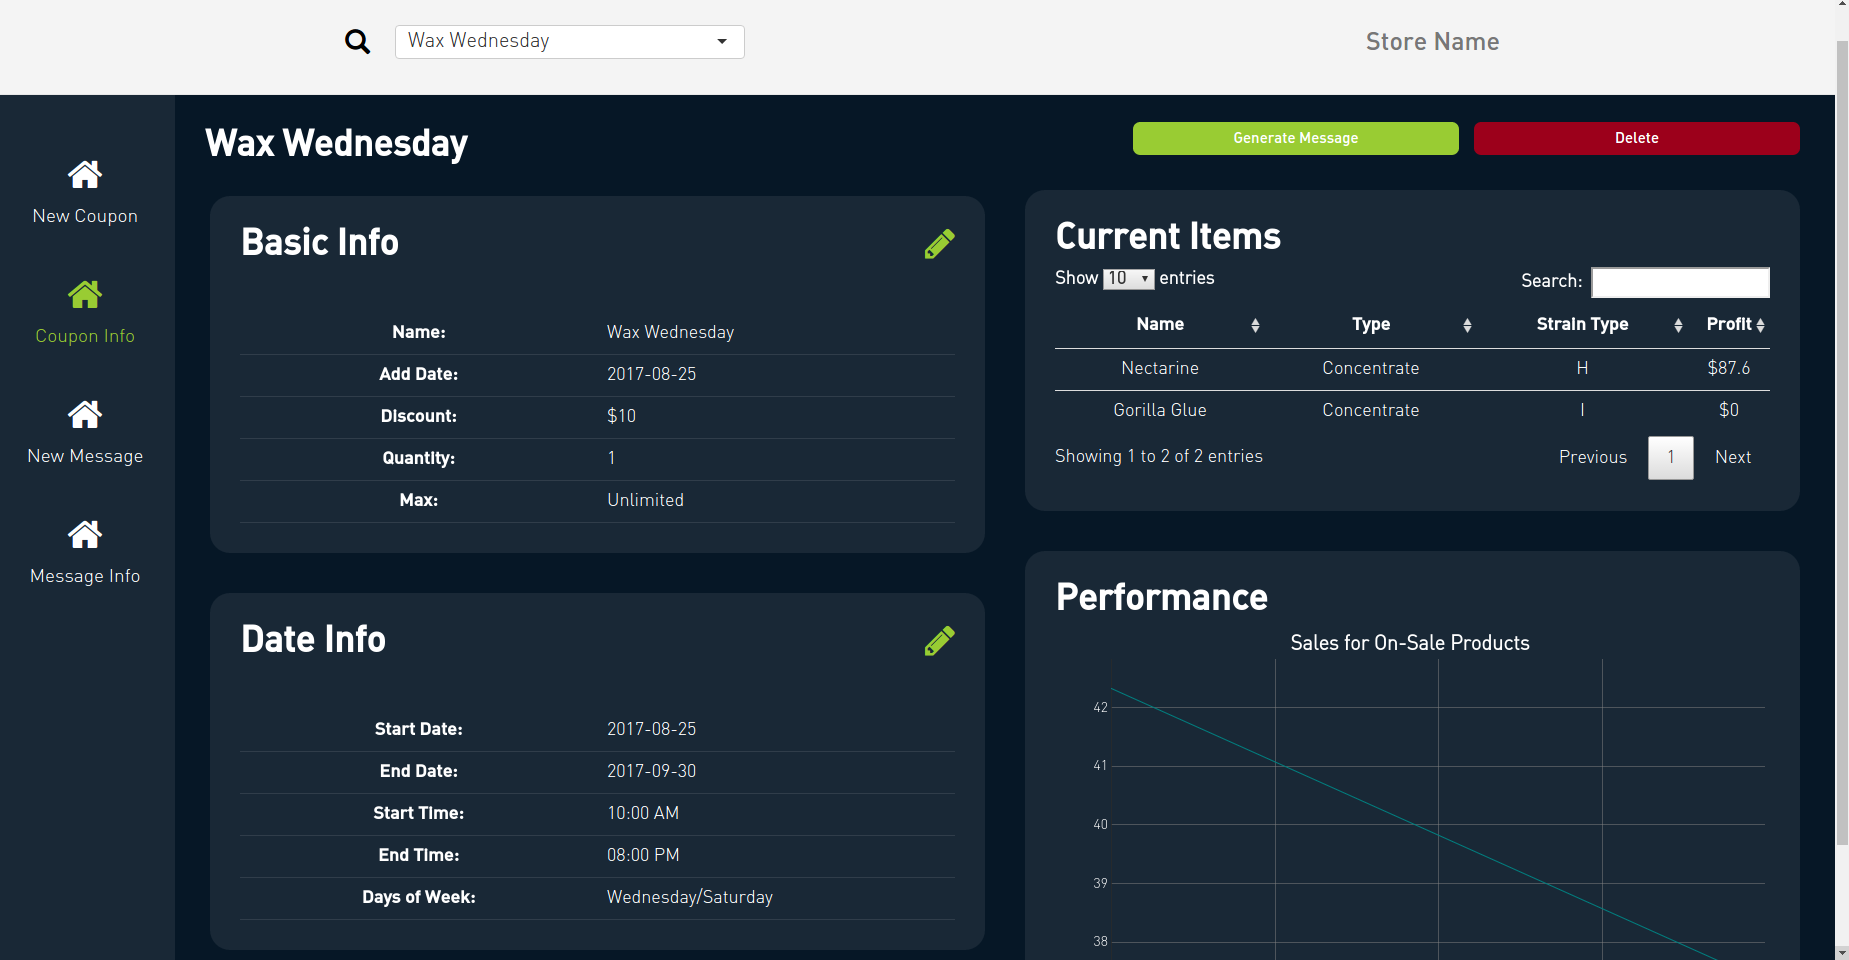
\includegraphics{images/C4.png}
\caption{Info for Wax Wednesday}
\end{figure}

\section{Messages}\label{messages}

\subsection{New Messages}\label{new-messages}

To send a new message out to patients you are required to enter:

\begin{itemize}
\item
  A name
\item
  Message type (text or email)
\item
  Audience (based on patient preferences)
\item
  The message
\item
  If you send an email a subject is required
\end{itemize}

\begin{figure}
\centering
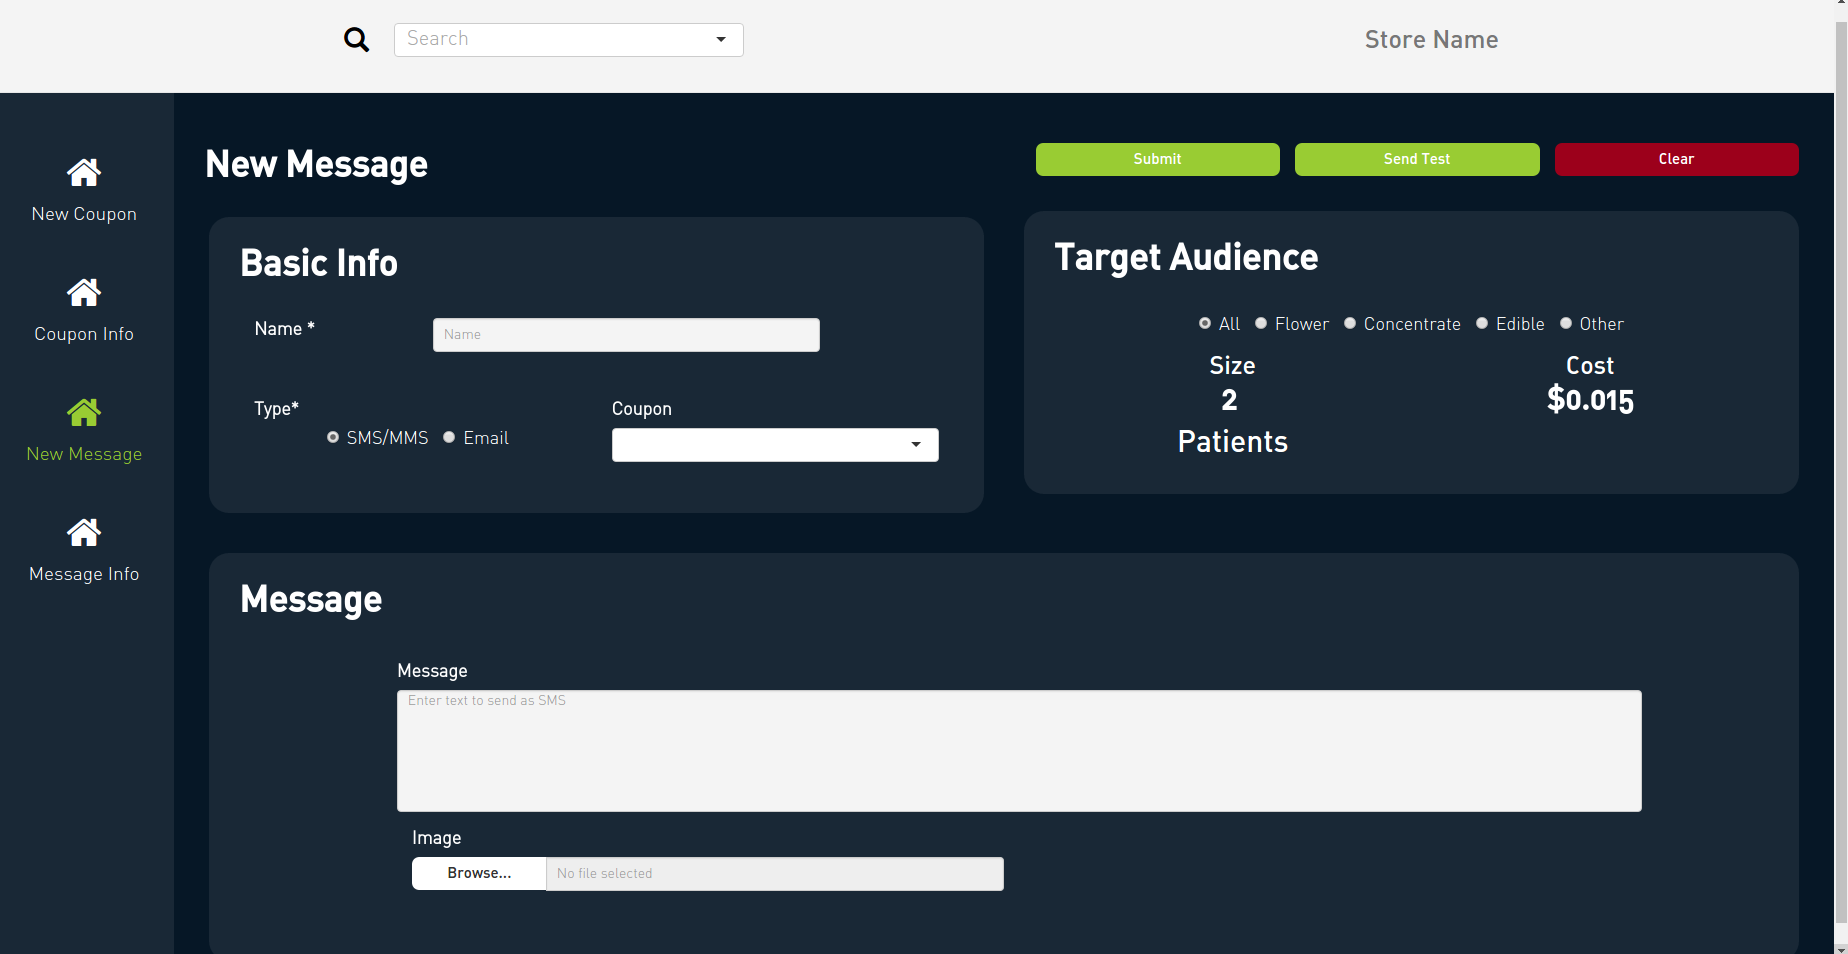
\includegraphics{images/C5.png}
\caption{New Text Message}
\end{figure}

\begin{figure}
\centering
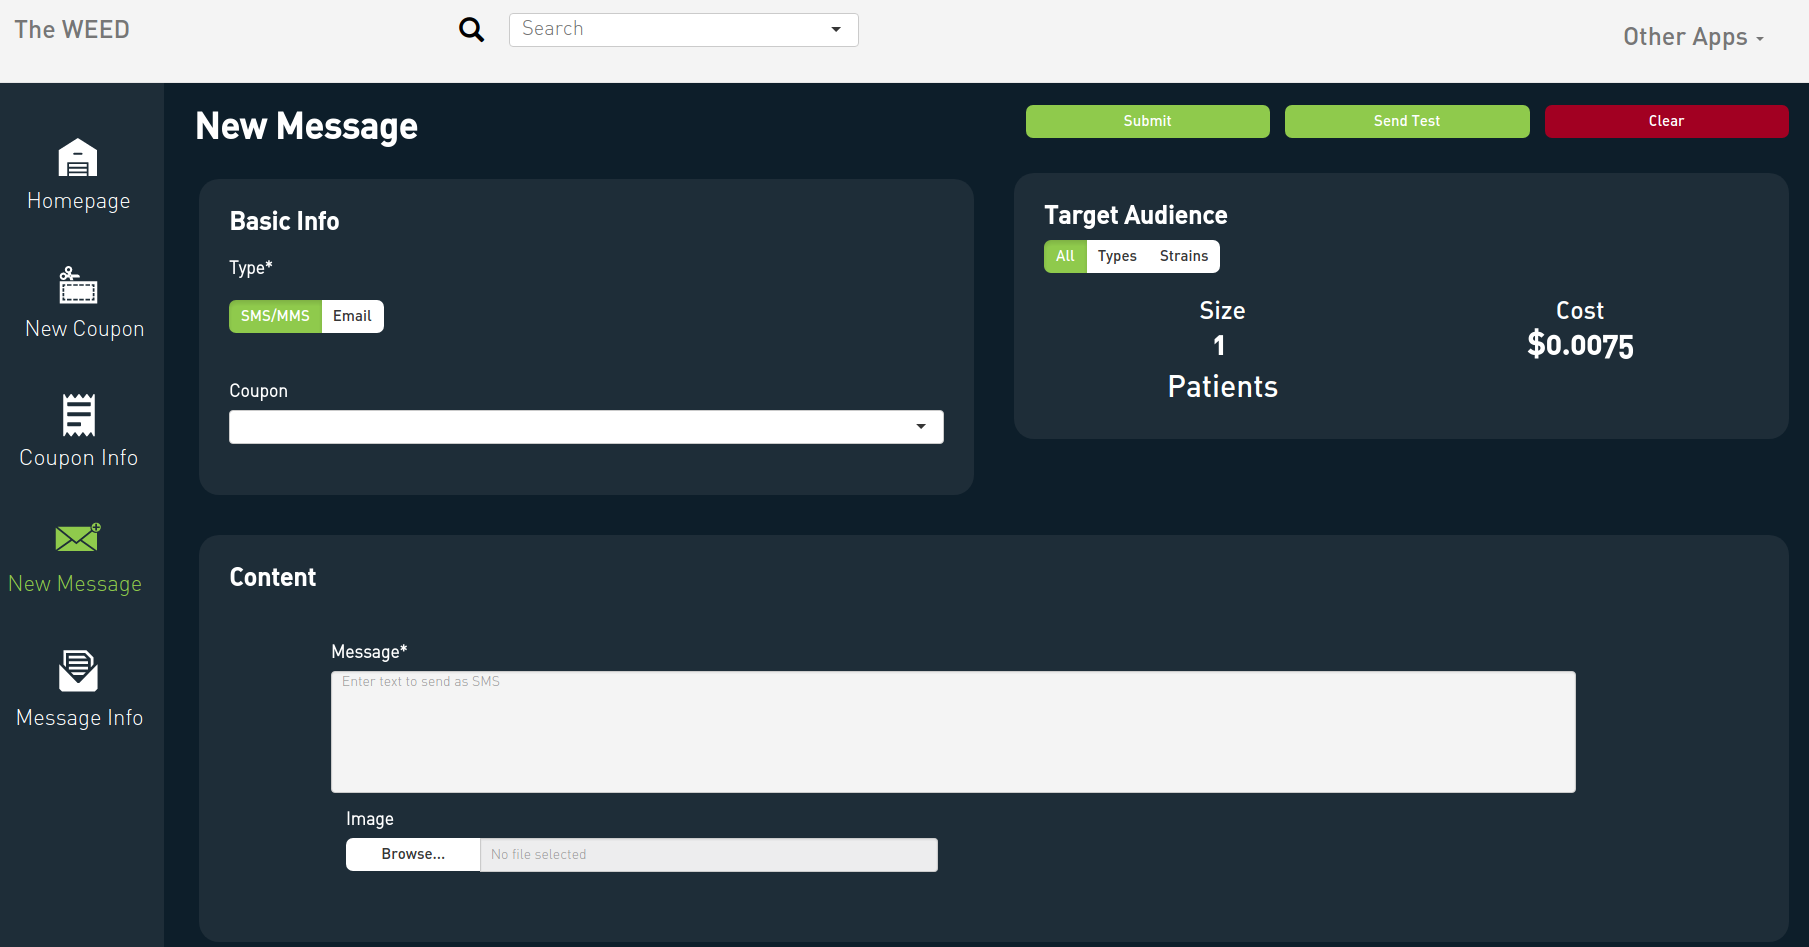
\includegraphics{images/C6.png}
\caption{New Email}
\end{figure}

\subsection{Message Info}\label{message-info}

You can review the info about past messages by selected the message in
the search box at the top. This will give you basic info about the
message like when it was sent, to whom, and its content. There is also a
graph of daily sales of the patients who were messaged, which makes it
easy to check whether the message let to a noticable increase in sales.

\begin{figure}
\centering
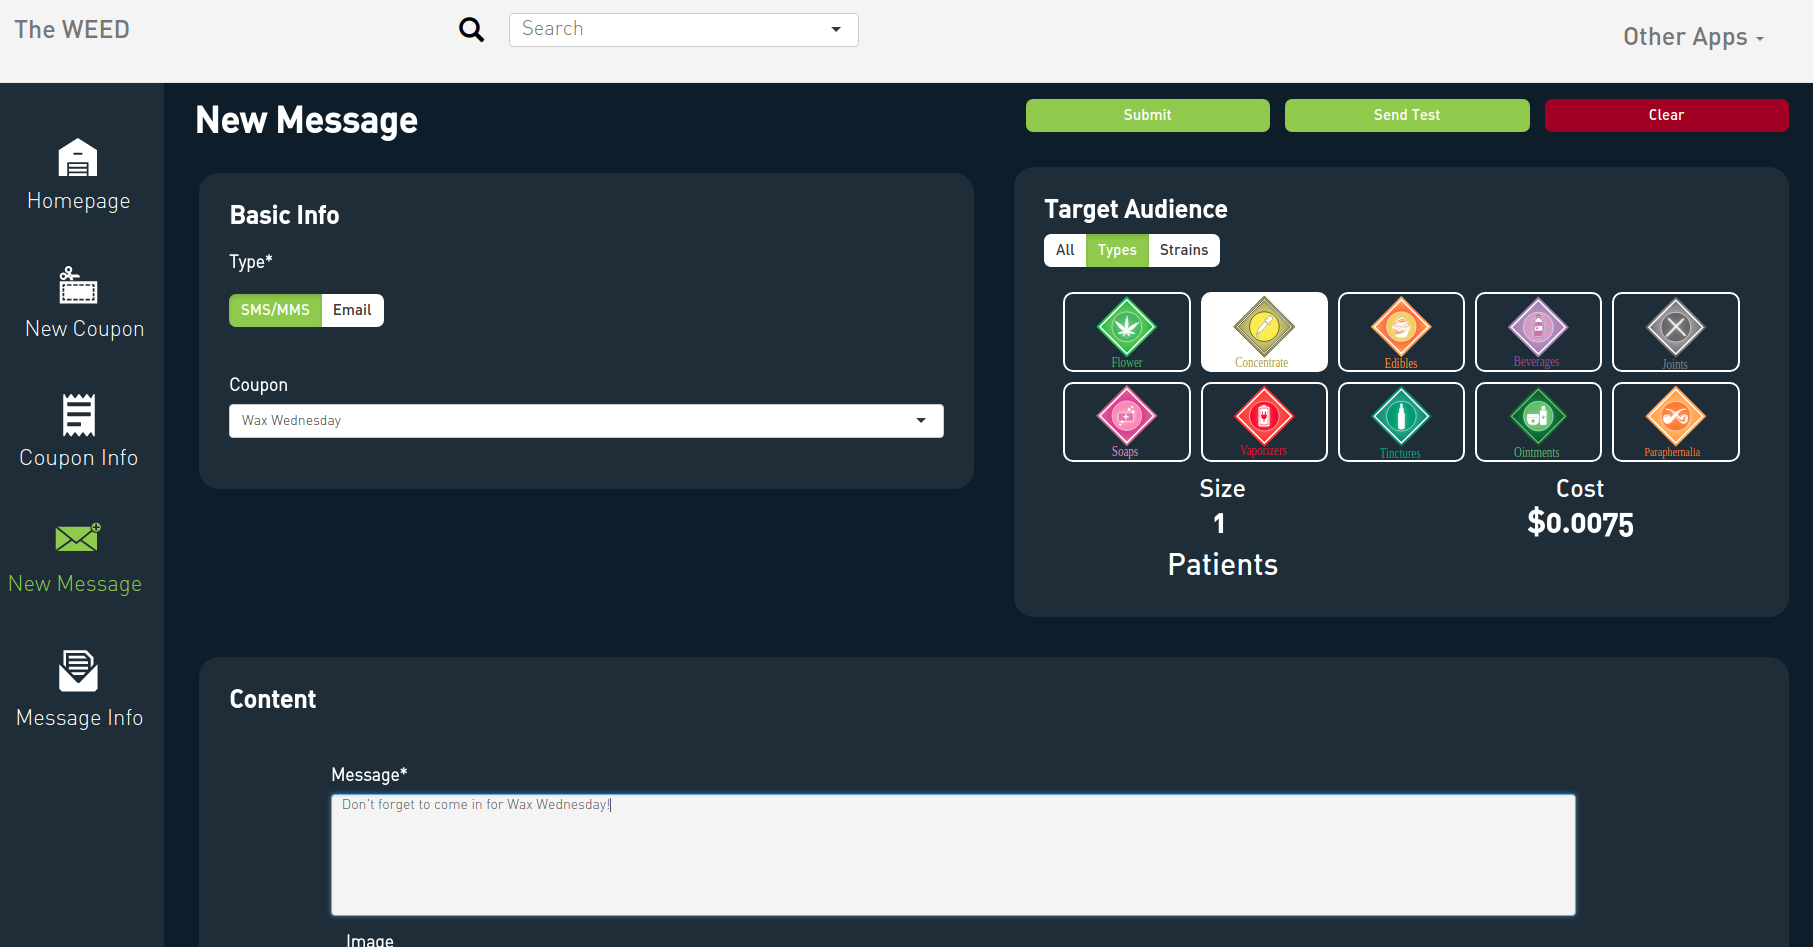
\includegraphics{images/C7.png}
\caption{Message Info for Wax Alert}
\end{figure}

\chapter{Point of Sales}\label{point-of-sales}


\end{document}
